\documentclass[letterpaper,titlepage,12pt,draft]{report}
%\usepackage[latin1]{inputenc}
\usepackage[utf8]{inputenc}
\usepackage[spanish]{babel}
\usepackage[pdftex]{graphicx}
\usepackage{graphicx}
\usepackage{float}
\usepackage{amssymb,amsfonts,amsmath,latexsym,theorem}
\usepackage{amsfonts}
\usepackage{tabularx}
\usepackage[usenames]{color}
\usepackage[table,xcdraw]{xcolor}

\newtheorem{definition}{Definici\'on}
\newtheorem{theorem}{Teorema}
\newtheorem{Example}{Ejemplo}
\newtheorem{Exercise}{Ejercicio}
\newtheorem{proposition}{Proposici\'on}
\newtheorem{lemma}[theorem]{Lema}
\newenvironment{proof}[1][Demostraci\'on]{\textbf{#1.} }{\rule{0.1cm}{0.1cm}}
\newtheorem{remark}{Obsevaci\'on}
\newtheorem{example}[theorem]{Ejemplo}
\newtheorem{corollary}{Corolario}
\usepackage[none]{hyphenat} %evitar malos cortes de silabas

\begin{document}
\sloppy %evitar malos cortes de silabas
%----------------------------------------------------------------Portada-----------

\begin{center}

\includegraphics[width=3cm]{Escudo.jpg}\\
\textsf{Universidad Aut\'onoma del Estado de Hidalgo}\\
\textsf{Instituto de Ciencias B\'asicas e Ingenier\'ia}\\
\textsf{Centro de Investigaci\'on en Matem\'aticas}\\
\textsf{---------------------------}\\
\vspace{1cm} {\Huge {\bf El color del ruido en el sue\~no}}\\
\vspace{2mm}   {\Huge {\bf MOR de adultos mayores con y sin deterioro cognitivo}}\\
\vspace{1cm} {Tesis para obtener el t\'itulo de:}\\
\vspace{0.5cm} {\Large Licenciada en Matem\'aticas Aplicadas}\\
\vspace{1cm} {presenta:}\\
\vspace{0.5cm} {\Large Valeria Garc\'ia Mu\~noz}\\
\vspace{1cm} {bajo la supervisi\'on de:}\\ 
\vspace{0.3cm} {\large Dra. Erika Elizabeth Rodr\'iguez Torres}\\
\vspace{3mm} {\large Dr. Pedro Eduardo Miramontes Vidal}\\
\vspace{1cm} {\textsc Mineral de la Reforma, Hidalgo. Mayo de 2018.}
\end{center}

\pagenumbering{roman}

%------------------------------------------------------------------Agradecimientos-------------
\newpage

%\chapter*{Agradecimientos} % si no queremos que a�ada la palabra "Capitulo"
%\addcontentsline{toc}{chapter}{Agradecimientos} % si queremos que aparezca en el �ndice
%\markboth{AGRADECIMIENTOS}{AGRADECIMIENTOS} % encabezado

%-----------------------
\newpage
\chapter*{Siglas}

\begin{itemize}
\item[{\bf AM}] Adulto mayor
\item[{\bf DC}] Deterioro cognitivo
\item[{\bf DFA}] Detrended Fluctuation Analysis / An\'alisis de fluctuaci\'on sin tendencia
\item[{\bf mDFA}] multifractal Detrended Fluctuation Analysis / An\'alisis de fluctuaci\'on sin tendencia multicanal
\item[{\bf EEG}] Electroencefalograma / Electroencefalograf\'ia 
\item[{\bf EMG}] Electromiograma / Electromiograf\'ia
\item[{\bf EOG}] Electrooculograma / Electrooculograf\'ia
\item[{\bf MOR}] Movimientos oculares r\'apidos
\item[{\bf PSG}] Polisomnograma / Polisomnograf\'ia
\end{itemize}

%------------------------------------------------------------------
\newpage
\begin{center}
\chapter*{Resumen}
\addcontentsline{toc}{section}{\bf Resumen}% Aparece en el �ndide pero no como cap�tulo
\end{center}

Se acepta ampliamente que los EEG de adultos mayores con o sin deterioro cognitivo deben ser diferentes. Por lo que en este trabajo utilizamos herramientas de an\'alisis de series de tiempo no lineales para evaluar cuantitativamente tales diferencias. Espec\'ificamente, empleamos el color del ruido para conocer la diferencia.\\

\vspace{2cm}
\begin{flushleft}
{\bf {\huge Abstract}}\\
\end{flushleft}
\vspace{1cm}

It is widely accepted that EEGs from the elderly with and without cognitive impairment should be
different. In this study we used tools from nonlinear time series analysis to quantitatively
assess the difference. Specifically, the evaluation of the color of the noise in time series has
shown to be a valuable tool to distinguish the difference.

%------------------------------------------------------------------------�ndice--------
\newpage
\tableofcontents
\cleardoublepage

%---------------------------------------------------------------------Introducci�n--Primer cap�tulo---
\newpage
\pagenumbering{arabic} % para empezar la numeraci�n con n�meros
\chapter*{Introducci\'on} %
\addcontentsline{toc}{section}{\bf Introducci\'on}% Aparece en el �ndide pero no como cap�tulo

El diagn\'ostico cl\'inico y las investigaciones b\'asicas dependen fundamentalmente de la capacidad de registrar y analizar las se\~nales biol\'ogicas, sin embargo, los an\'alisis tradicionales de las se\~nales registradas en laboratorio no han seguido el ritmo de los mayores avances tecnol\'ogicos que permiten el registro y almacenamiento de conjuntos de datos masivos de se\~nales fluctuantes continuas. Aunque recientemente se ha demostrado que estas se\~nales t\'ipicamente complejas representan procesos que son no lineales y no estacionarios, las herramientas para analizar tales datos a menudo siguen asumiendo linealidad y estacionalidad. A consecuencia de lo anterior, dichos conjuntos de datos pueden contener informaci\'on oculta, la cual puede ser de valor cl\'inico. En este trabajo de tesis se pretende usar una herramienta matem\'atica que involucra la no linealidad.\\

 El an\'alisis fractal es un nuevo enfoque y de los m\'as prometedores para extraer informaci\'on oculta. La cual ayudar\'a a tener una idea m\'as clara de lo que puede ocurrir a largo plazo, o bien de los cambios que se est\'an presentando en los diferentes contextos de manera m\'as clara y sencilla, con resultados concretos y exactos. Proporcionando as\'i una herramienta, que permita mostrar cambios en las distintas maniobras experimentales o en aplicaciones cl\'inicas con distintas patolog\'ias.\\
 
El principal objetivo de este trabajo es encontrar las diferencias significativas entre los registros obtenidos a trav\'es polisomnograf\'ias de adultos mayores con y sin deterioro cognitivo. Ya que se ha demostrado que las se\~nales registradas en pacientes sanos pueden caracterizarse de acuerdo a un color del ruido, el cual se define como el color rosa, mientras que con pacientes con alguna anomal\'ia neurol\'ogica pueden presentar un color del ruido caf\'e, esto se define con m\'as detalle en la siguiente secci\'on.
%----------------------
\newpage
\chapter{Planteamiento del problema}

\section{Justificaci\'on}

El crecimiento acelerado de la poblaci\'on adulta a nivel mundial, de acuerdo con la Organizaci\'on de las Naciones Unidas, en 2025 habr\'a m\'as de 1,100 millones de personas de entre 60 a\~nos o m\'as en todo el mundo; por lo cual se ha vuelto un tema de inter\'es para la Organizaci\'on Mundial de la Salud\cite{OMS}, ya que debido a las modificaciones morfol\'ogicas, fisiol\'ogicas, bioqu\'imicas y psicol\'ogicas del envejecimiento\cite{ING}, se incrementa una probabilidad de padecer enfermedades cr\'onicas.\\

En particular el deterioro cognitivo, es un estado intermedio entre normalidad y demencia senil, afectando la calidad de vida de los adultos mayores y generando costos para la familia y la sociedad. Por ello, existe la necesidad de que en el sistema de salud, realice una valoraci\'on integral del adulto mayor por parte del equipo de salud, para la detecci\'on temprana del deterioro cognitivo ya que al no ser diagnosticado adecuadamente incrementa el riesgo de evolucionar a demencia y por consiguiente largos y pesados periodos de cuidado y una atenci\'on especializada para recibir el tratamiento m\'as apropiado al que no todos tienen acceso, por los gastos que representa en todos los niveles.\\

Existen diferentes herramientas matem\'aticas que pueden ser implementadas a casos biol\'ogicos, las cuales no necesariamente est\'an regidas por la geometr\'ia euclidiana, sino por la geometr\'ia fractal, herramientas que se han usado para detectar tanto patrones como diferencias significativas en estudios fisiol\'ogicos{\cite{cartel}}{\cite{carteloli}}.\\

A\'un no hay trabajos enfocados al an\'alisis de \'epocas de sue\~no MOR en adultos mayores, por lo cual, el presente trabajo esta enfocado en mostrar que existen diferencias significativas entre los registros de adultos mayores con deterioro cognitivo de los que no. Donde a trav\'es de un an\'alisis efectuado a cada una de las se\~nales, se podr\'a clasificar el color del ruido de la misma, permitiendo ver una relaci\'on entre el deterioro cognitivo y el sue\~no MOR de los adultos mayores, m\'etodo con el cual se pretende tener una justificaci\'on sobre tal relaci\'on. Con lo cual se tendr\'a un beneficio para la comunidad adulta, permitiendo prevenir casos posteriores de deterioro cognitivo, llevando a cabo esta prueba, y a su vez prevenir demencias y otras enfermedades que esto puede generar a futuro. 

\section{Pregunta de investigaci\'on}

Existen diferencias significativas entre los canales y las correlaciones interhemisf\'ericas del sue\~no MOR de adultos mayores con y sin deterioro cognitivo?\\

Donde se tiene las siguientes hip\'otesis:\\

H1: Existen diferencias estad\'isticamente significativas en la correlaci\'on interhemisf\'erica o el tono muscular del sue\~no MOR entre las personas que presentan deterioro cognitivo mostrando un ruido browniano, comparadas con aquellas que no tienen deterioro cognitivo, presentan tendencia al ruido rosa.\\

H0: No existen diferencias estad\'isticamente significativas en la correlaci\'on interhemisf\'erica o el tono muscular del sue\~no MOR entre las personas que presentan deterioro cognitivo mostrando un ruido browniano, comparadas con aquellas que no tienen deterioro cognitivo, presentan tendencia al ruido rosa.

%-------------------------

\section{Objetivo general}
Comparar la correlaci\'on interhemisf\'erica durante el sue\~no MOR de adultos mayores con y sin deterioro cognitivo, y probar que hay una tendencia al color rosa para aquellos sin deterioro cognitivo y hacia el ruido browniano para quienes tienen deterioro cognitivo, adem\'as de mostrar que el tono muscular presencia un ruido blanco.

\section{Objetivos particulares}
\begin{itemize}
\item Determinar el an\'alisis de fluctuaci\'on sin tendencia (\textit{Detrended Fluctuation Analysis}, DFA)  de cada canal de las \'epocas de sue\~no MOR de adultos mayores con DC y sin DC.
\item Determinar el an\'alisis de fluctuaci\'on sin tendencia multicanal (\textit{multifractal Detrended Fluctuation Analysis}, mDFA) de la polisomnograf\'ia de las \'epocas de sue\~no MOR.
\item Dados los resultados del DFA y mDFA, relacionarlos con el color del ruido, seg\'un les corresponda. 
\item Comparar los resultados de adultos mayores con DC versus adultos mayores sin DC. 
\item Realizar el mismo an\'alisis para m\'as sujetos y promediar los resultados. 
\end{itemize}
%--------------------


\chapter{El color del ruido}

\section{Espectro}

Comenzaremos definiendo que es una onda y los elementos que la componen, ya que ser\'an necesarios para la definici\'on de espectro de frecuencia.\\

Una onda consiste en la propagaci\'on de una perturbaci\'on de alguna propiedad del espacio, implicando un transporte de energ\'ia sin transporte de materia. Intuitivamente se llama onda al transporte de perturbaciones en el espacio, donde se considera el espacio como un medio en el que puede producirse y propagarse dichas perturbaciones. La cual esta compuesta por:
\begin{itemize}
\item{\bf Cresta:} m\'axima amplitud de onda, es decir, el punto de la onda m\'as separado de su posici\'on de reposo. 
\item{\bf Valle:} punto m\'as bajo de una onda.
\item{\bf Amplitud:} distancia vertical entre una cresta y el punto medio de la onda.
\item{\bf Frecuencia ($f$):} n\'umero de veces que es repetida dicha vibraci\'on por unidad de tiempo.
\item{\bf Periodo ($T$):} tiempo que tarda la onda en ir de un punto de m\'axima amplitud al siguiente. $$T=\frac{1}{f}$$
\item{\bf Longitud de onda ($\lambda$):} distancia que hay entre el mismo punto de dos ondulaciones consecutivas, o la distancia entre dos crestas consecutivas.
\item{\bf Nodo:} punto donde la onda cruza la l\'inea de equilibrio.
\item{\bf Elongaci\'on:} distancia que hay, en forma perpendicular, entre un punto de la onda y la l\'inea de equilibrio.
\item{\bf Ciclo:} es una oscilaci\'on, o el recorrido desde la cresta al valle o viceversa.
\item{\bf Velocidad de propagaci\'on ($v$):} velocidad a la que se propaga el movimiento ondulatorio.$$v=\frac{\lambda}{T}$$
\end{itemize}

\begin{figure}[H]
\begin{center}
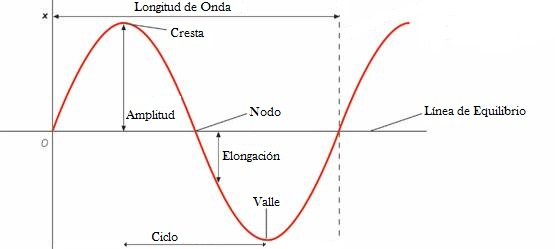
\includegraphics[scale=0.5]{onda.jpg}
\caption{Componentes de la onda.}
\label{fig:onda}
\end{center}
\end{figure}

En cuando a la palabra {\bf espectro}, este puede referirse a diferentes conceptos, sin embargo solo se consideraran los t\'erminos empleados para el trabajo realizado.

\subsection{Espectro de frecuencias}

Se define al {\bf espectro de frecuencia}, tambi\'en llamado {\bf descomposici\'on espectral de frecuencias}, a la distribuci\'on de amplitudes para cada frecuencia de un fen\'omeno ondulatorio (sonoro, luminoso o electromagn\'etico) que sea superposici\'on de ondas de varias frecuencias. O bien el gr\'afico de intensidad frente a frecuencia de onda particular. \\

\begin{figure}[H]
\begin{center}
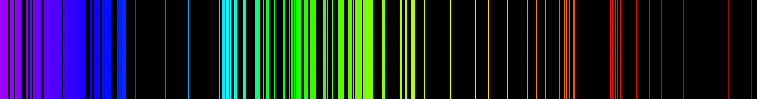
\includegraphics[scale=0.5]{ef.png}
\caption{Espectro de frecuencias de la luz emitida por \'atomos de hierro libres en la regi\'on visible del espectro electromagn\'etico.}
\label{fig:ef}
\end{center}
\end{figure}

Puesto que el an\'alisis se refiere a la acci\'on de descomponer algo complejo en partes simples, llamaremos al an\'alisis espectral como el proceso que cuantifica las diversas intensidades de cada frecuencia. 

\subsection{Espectro electromagn\'etico}

El {\bf espectro electromagn\'etico} se refiere al conjunto de las ondas electromagn\'eticas, es decir, a la radiaci\'on electromagn\'etica que emite o absorbe una sustancia.

\begin{figure}[H]
\begin{center}
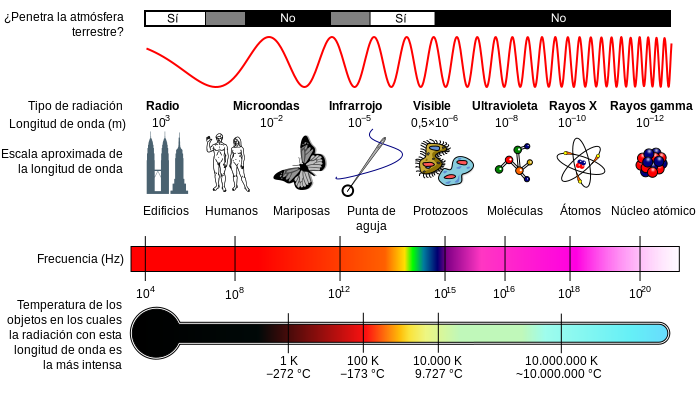
\includegraphics[scale=0.5]{ee.png}
\caption{Diagrama del espectro electromagn\'etico, mostrando el tipo, longitud de onda con ejemplos, frecuencia y temperatura de emisi\'on de cuerpo negro.}
\label{fig:ee}
\end{center}
\end{figure}

\section{El Color del ruido}

Por lo anterior es posible notar la naturaleza ondulatoria de la luz, donde cada uno de los colores que componen el espectro continuo corresponde a una frecuencia de oscilaci\'on electromagn\'etica o una longitud de onda como en la Figura \ref{fig:color}, por ejemplo: Amarillo=600 nan\'ometros, Rojo=650 nan\'ometros o el Violeta=380 nan\'ometros.\\

\begin{figure}[H]
\begin{center}
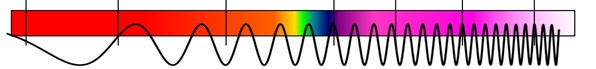
\includegraphics[scale=0.5]{espectro_onda.jpg}
\caption{Relaci\'on entre el color y la frecuencia de oscilaci\'on.}
\label{fig:color}
\end{center}
\end{figure}

Se le llama {\bf color del ruido} a la relaci\'on que existe entre las ondas de luz y las del ruido. Es decir, el ruido con un espectro de potencia que varia con la frecuencia. \cite{Miramontes}\\

Por lo anterior es natural considerar que cualquier serie de tiempo, independiente de su origen, tiene un espectro de potencia determinado por la transformada de Fourier. En la mayor\'ia de las series de tiempo biol\'ogicas se muestra una curva finita cuando el espectro de potencia es graficado con respecto a la frecuencia. Cuando la curva decrece, se representa por la funci\'on: 

\begin{equation}
1/f^{\alpha}
\label{potencia}
\end{equation}

Los diferentes tipos de color del ruido dependen de la norma del espectro de potencia y de la distribuci\'on de los valores. Para este trabajo se tiene un inter\'es principal cuando $\alpha$ es negativo, desde el trabajo seminal de George Kingsley Zipf, quien encontr\'o que la frecuencia de cualquier palabra trazada contra su rango es una ley de potencias con exponente $\alpha=-1$.\\


{\bf Ruido Blanco}\\

Conocido tambi\'en como ruido blanco Gaussiano, es la combinaci\'on de todos los colores. Con $\alpha\approx0$ ($\frac{1}{f^0}$) significa que est\'an presentes todas las frecuencias de los agentes individuales posibles. \\

El ruido blanco se caracteriza adem\'as por la distribuci\'on de valores en la serie de tiempo. Donde al elegir los valores de manera aleatoria entre el 0 y el 1, \'estos tienen una distribuci\'on normal (o Gaussiana), la cual es importante  porque surge de varios procesos de la naturaleza. Algunos ejemplos son la est\'atica de los radios antiguos, tocar notas distintas sin coordinaci\'on, ninguna periodicidad ni patr\'on.\\

%{\bf Ruido Rojo}\\
%
%Se caracteriza por frecuencias altas. Por ejemplo: oceanograf�a o fluctuaciones de un d�a del �ndice de precios. \\
%
%{\bf Ruido Azul}\\
%
%Absorbe las frecuencias bajas.\\
%
%{\bf Ruido Gris}\\
%
%Cada componente tiene la misma energ�a y su funci�n es decreciente.\\

{\bf Ruido Browniano}\\

Llamado as\'i por ser equivalente al movimiento Browniano, cuyo nombre viene de Robert Brown, el cual no tiene relaci\'on alguna con el color, sin embargo es conocido y llamado como ruido caf\'e. Donde dada una serie de n\'umeros azarosa, el espectro disminuye como una hip\'erbola trazada por $\frac{1}{f^2}$. \\

%{\bf Ruido Negro}\\
%
%Manfred Schoeder, determino su hip�rbola como $\frac{1}{f^3}$. Donde el dominio de las frecuencias bajas est�n sobre las altas. Caracter�stico de los desastres naturales y artificiales como inundaciones o apagones.  As� como lo que no podemos ver o escuchar, es decir como los rayos ultravioleta o bien los silbatos para perros.\\

{\bf Ruido Rosa}\\

Tambi\'en conocido como el ruido biol\'ogico o ruido de Centelleo o color de la vida. Es una combinaci\'on del ruido rojo (frecuencias bajas entran en mayor proporci\'on que las altas) con el ruido blanco (todas las frecuencias representadas). La hip\'erbola que traza esta dada por $\frac{1}{f^1}$. Con coordenadas logar\'itmicas, recta de pendiente negativa y cercana a la unidad. Es una indicaci\'on de que el fen\'omeno tiene un origen din\'amico, es decir, no es aleatorio.\\

Omnipresente en la naturaleza. No existe una explicaci\'on te\'orica de la raz\'on de su ubicuidad en la naturaleza, por lo que en 1987 Per Bak: lo llama el color de la vida. Como un sistema del equilibrio generan estructuras y patrones sin necesidad de agentes externos.\\

Los sistemas din\'amicos formados por un gran n\'umero de componentes no lineales tiene una tendencia espont\'anea a organizarse a s\'i mismos en estados cr\'iticos de equilibrio din\'amico, donde ocurren fluctuaciones de todos los tama\~nos. Con relaci\'on a las se\~nales fisiol\'ogicas existen tres ruidos de inter\'es con los que \'estas se pueden clasificar, entre los que se encuentran: el ruido blanco, que es una combinaci\'on de todas las colores; el ruido caf\'e, conocido como ruido Browniano y por \'ultimo el ruido rosa. 
%---------------------

\chapter{Contexto biol\'ogico}
%-------------------------------------------------------------------------------

\section{Adulto mayor}
Un adulto mayor, de acuerdo a la Organizaci\'on Mundial de la Salud, son aquellas personas de 60 a 74 a\~nos y son considerados de edad avanzada, de 75 a 90 viejas o ancianas, y las que sobrepasan los 90 se les denomina grandes viejos o longevos. A todo individuo mayor de 60 a\~nos se le llamar\'a indistintamente persona de la tercera edad o adulto mayor.


\section{Deterioro cognitivo}

Se le llama Deterioro Cognitivo (DC) a la presencia de quejas subjetivas de memoria con correspondientes dificultades en pruebas objetivas pero con conservaci\'on del funcionamiento cognitivo general y sin se\~nales de alteraci\'on en el funcionamiento de las actividades de la vida diaria que impidan una vida independiente\cite{DC}. De acuerdo a las variaciones en el nivel de severidad del DC este se subdivide en los siguientes tipos:

\begin{itemize}
\item {\bf DC cl\'asico:} Afecta \'unicamente en la memoria.
\item {\bf DC moderado:} Aparte de haber una alteraci\'on en la memoria, \'este incluye la atenci\'on, el lenguaje, funciones ejecutivas o funciones visoespaciales.
\item {\bf DC severo:} Transtornos en al menos dos dominios cognitivos.
\end{itemize}


\section{El sue\~no}

El sue\~no es una parte integral de la vida cotidiana, una necesidad biol\'ogica que se basa en un estado fisiol\'ogico, activo, c\'iclico y reversible (lo que lo diferencia del estado de coma), compuesto por varias fases y diferentes interrelaciones en los sistemas hormonales y nerviosos \cite{Conde}.\\

Este se determina por cuatro dimensiones diferentes: tiempo circadiano (la hora del d\'ia en el que se realiza); factores intr\'insecos del organismo (edad, sexo, patrones de sue\~no, estado fisiol\'ogico, etc.); conductas que facilitan o inhiben el sue\~no y por \'ultimo el ambiente. Donde las dos \'ultimas se relacionan con la higiene del sue\~no que incluye las pr\'acticas necesarias para mantener un sue\~no nocturno y una vigilancia diurna normales \cite{Sierra}.\\

Durante este proceso conocido como sue\~no los seres vivos tienen su propio ritmo de actividad y reposo, el hipot\'alamo (gl\'andula hormonal que controla y regula cada gl\'andula y a la vez cada una de las funciones del organismo) se encuentra relacionado con el sentido neurol\'ogico de la ritmicidad del sue\~no. Por lo cual existen diversas teor\'ias acerca de las funciones del sue\~no, dentro de las cuales est\'an:

\begin{itemize}
\item Restablecimiento o conservaci\'on de la energ\'ia.
\item Eliminaci\'on de radicales libres acumulados durante el d\'ia.
\item Regulaci\'on y restauraci\'on de la actividad el\'ectrica cortical
\item Regulaci\'on t\'ermica.
\item Regulaci\'on metab\'olica y endocrina.
\item Homeostasis sin\'aptica.
\item Activaci\'on inmunil\'ogica.
\item Consolidaci\'on de la memoria. 
\end{itemize}

%--------------------------------------
\section{Etapas del sue\~no}

El sue\~no normal se divide en dos etapas: sue\~no REM (\textit{Rapid-Eye-Movement}) o tambi\'en conocido como sue\~o MOR (movimiento ocular r\'apido) y sue\~no no REM, los cuales se diferencian fundamentalmente por sus rasgos electroencefalogr\'aficos y una serie de caracter\'isticas fisiol\'ogicas \cite{et_sue}. Mediante los estudios polisomnogr\'aficos se estudian los indicadores del sue\~no, los cuales permiten diferencia las distintas etapas del sue\~no, los cuales se mencionan a continuaci\'on:

\begin{itemize}
\item Electroencefalograma (EEG): Representaci\'on gr\'afica y digital de las oscilaciones que muestra la actividad el\'ectrica del cerebro, al ser registrada mediante electrodos colocados encima de la piel cabelluda en distintas regiones de la cabeza.
\item Movimientos oculares
\item Tono muscular
\end{itemize}

%--------------------------------------
\subsection{Sue\~no no MOR}

Las caracter\'isticas del sue\~no no MOR est\'an divididas en cuatro fases, cuya nomenclatura ha sido recientemente modificada por la Academia Americana de Medicina del Sue\~no (2007). Quedando de la siguiente forma:

\begin{itemize}
\item[N1:] (Fase 1) Corresponde a la transici\'on de la vigilia al sue\~no, la actividad muscular disminuye paulatinamente y pueden observarse algunas breves sacudidas musculares s\'ubitas que a veces coinciden con una sensaci\'on de ca\'ida. 
Frecuencias mezcladas, pero de bajo voltaje y algunas ondas agudas en el EEG.
\item[N2:] (Fase 2) Intermedia, mayor porcentaje del tiempo de sue\~no, la temperatura, la frecuencia cardiaca y respiratoria comienzan a disminuir paulatinamente.
En el EEG aparecen patrones espec\'ificos de actividad cerebral llamados husos de sue\~no y complejos K.
\item[N3:] (Fase 3 y 4) Sue\~no profundo o fase reparadora del sue\~no, aquella que produce en la persona la sensaci\'on de haber descansado cuando se levanta. En el EEG se observa actividad de frecuencia muy lenta\cite{sue}. 
\end{itemize}

Despu\'es de pasar por estas etapas, durante unos 70 a 120 minutos, suele presentarse la primera fase del Sue\~no MOR. 
%--------------------------------------	
\subsection{Sue\~no MOR}

Ahora llamado Fase R, el sue\~no MOR se caracteriza por:

\begin{itemize}
\item Movimientos musculares r\'apidos.
\item Aton\'ia muscular (con excepci\'on de los m\'usculos respiratorios y los esf\'interes vesical y anal)
\item La frecuencia card\'iaca y respiratoria se vuelve irregular e incluso puede incrementarse y existe erecci\'on espont\'anea del pene o del cl\'itoris.
\item Presencia de ondas de bajo voltaje y alta frecuencia en el EEG.
\end{itemize}

Durante el sue\~no MOR se presentan la mayor\'ia de los enso\~naciones (sue\~nos), y la mayor\'ia de los que despiertan durante esta fase tienen m\'as probabilidad de recordar el contenido de sus sue\~nos.\\

El sue\~no MOR ocupa el $20\%$ del sue\~no en el adulto, es decir, puede durar de 5 a 30 minutos, el ciclo de sue\~no no MOR y sue\~no MOR se repite aproximadamente cada hora y media durante toda la noche de sue\~no, presentando un total de 4 a 6 ciclos de sue\~no MOR normalmente, aunque \'estos var\'ian de acuerdo a la edad y las circunstancias individuales.\\

Un ni\~no reci\'en nacido duerme casi todo el d\'ia, con una proporci\'on pr\'oxima al $50\%$ del denominado sue\~no activo, que es el equivalente del sue\~no MOR. A lo largo de la lactancia los per\'iodos de vigilia son progresivamente m\'as prolongados y se consolida el sue\~no de la noche; adem\'as, la proporci\'on de sue\~no MOR desciende al $25-30\%$, que se mantendr\'a durante toda la vida. Entre el 1er y 3er a\~no de vida el ni\~no ya s\'olo duerme una o dos siestas. Entre los 4 y 5 a\~nos y la adolescencia los ni\~nos son hipervigilantes, muy pocos duermen siesta, pero tienen un sue\~no nocturno de 9-10 horas bien estructurado en 5 ciclos o m\'as. Por lo que se refiere a los individuos j\'ovenes, en ellos reaparece en muchos casos la necesidad fisiol\'ogica de una siesta a mitad del d\'ia\cite{Bonet}.\\

Por otro lado, en los ancianos se va fragmentando el sue\~no nocturno, reduci\'endose el porcentaje de sue\~no en la fase 4, y no tanto en el sue\~no MOR, el cual se mantiene constante a lo largo de la vida. 
 
%--------------------------------------
\section{Sue\~no y memoria}

Se ha demostrado que el sue\~no tiene efectos positivos sobre distintos tipos de memoria\cite{Vas}, espec\'ificamente en dos:

\begin{enumerate}
\item {\bf {La memoria declarativa:}} F\'acilmente expresada verbalmente, tales como hechos y eventos. La cu\'al es consolidad durante el Sue\~no No MOR (depende del hipocampo). 
\item {\bf {La memoria procedimental:}} Memoria acerca de las habilidades y destrezas motoras. Favorecida en el sue\~no MOR (independiente en el hipocampo).
\end{enumerate}

El sue\~no no s\'olo tiene un efecto sobre la informaci\'on aprendida previamente sino que tambi\'en mejora las capacidades de aprendizaje durante el d\'ia siguiente al periodo del sue\~no, en otras palabras el sue\~no previo tambi\'en mejora las habilidades diurnas de aprendizaje del d\'ia siguiente.

%--------------------------------------------------------------------------

\section{Cambios en la funci\'on cognitiva}
El deterioro progresivo de determinadas funciones cognitivas superiores es una de las caracter\'isticas del envejecimiento, sin embargo, otras capacidades cognitivas y sensorio motoras se mantienen relativamente conservadas en la \'ultima etapa de vida del  individuo. Al hablar de desarrollo cognitivo en el adulto mayor es imprescindible considerar la cognici\'on como un concepto multidimensional y multidireccional, dado que los cambios que se sufren durante esta etapa, afectan de diferente forma y se dan de manera distinta.\\

Los cambios cognitivos se dan en cualquier momento del desarrollo cognitivo de un individuo, ya que estos dependen de factores gen\'eticos, ambientales y sociales, adem\'as, todos los procesos del desarrollo suponen tanto p\'erdidas como ganancias y la mezcla que se refiere a factores socio culturales y bio-l\'ogicos cambia con la edad. Es decir, mientras que al principio predominan las ganancias, estas van cediendo con el paso del tiempo en campos concretos. Sin embargo, en edades superiores, pueden constatarse nuevos recursos, aunque no sean muy numerosos.\\

Por su parte Baltes\cite{Baltes} propone una diferencia durante el envejecimiento en los procesos cognitivos mentales, que si bien disminuyen, existen los que permanecen estables o incluso llegan a mejorar. De acuerdo con este autor, la mec\'anica cognitiva (la percepci\'on sensorial, la atenci\'on, la memoria visual y motora, as\'i como la discriminaci\'on, la comparaci\'on y la categorizaci\'on) puede disminuir con los a\~nos y la pragm\'atica cognitiva (habilidad para la lectoescritura, la comprensi\'on verbal, la formaci\'on educativa, las capacidades laborales y tambi\'en el tipo de conocimiento acerca de uno mismo) puede incluso, mejorar.

\section{Alteraciones en el sue\~no del adulto mayor}

Las alteraciones de sue\~no, espec\'ificamente en personas mayores se han asociado con la presencia de enfermedades cr\'onicas, problemas f\'isicos y de salud mental; asociadas directamente con una disfunci\'on cognitiva.\\

Es decir, tanto la privaci\'on del sue\~no como la mala calidad de \'este, son indicadores negativos sobre la somnolencia, el rendimiento motor y cognitivo e incluso sobre el humor o estado de \'animo produciendo irritabilidad, impaciencia, ansiedad, depresi\'on entre otros. Adem\'as de afectar funciones sobre el metabolismo, el funcionamiento hormonal y cognitivo de manera significativa.\\

Formando as\'i un inter\'es por analizar la relaci\'on entre el sue\~no y el deterioro cognitivo del adulto mayor, lo cual se abordar\'a en los siguientes cap\'itulos.


%-----------------------------------------------------------------------------
\newpage
\chapter{Metodolog\'ia}

La metodolog\'ia se divide en dos partes, la primera corresponde a los procedimientos (i.e. el m\'etodo biol\'ogico) para obtener las series de tiempo que se registraron en adultos mayores durante una noche de sue\~no, mientras que la segunda parte describe el m\'etodo matem\'atico para el an\'alisis de tales series.

%------------------------------------------------------------------------------------DFA-------------

\section{M\'etodo biol\'ogico}

Para este estudio los participantes, adultos mayores de 60 a\~nos o m\'as, comenzaran respondiendo los ex\'amenes \textit{Neuropsi} y \textit{Mini Mental State Examination}, cuyos resultados ser\'an interpretados por expertos para determinar si se ha encontrado que presentan deterioro cognitivo de dominio \'unico o de m\'ultiples dominios. (Psic\'ologa G\'enesis V\'azquez Tagle Gallegos y la Dra. Alejandra Rosales, UAEH) \\

Posteriormente cada participante acudir\'a, en este caso, a la Cl\'inica Gerontol\'ogica de Sue\~no ubicada en las instalaciones del Instituto de Ciencias de la Salud de la Universidad Aut\'onoma del Estado de Hidalgo alrededor de las 17:00h para la colocaci\'on de los electrodos, ya que este procedimiento tarda de entre 2 a 3 horas. La hora de comienzo del registro polisomnograf\'ia se adaptar\'a a la hora habitual de acostarse de cada sujeto.\\

El protocolo de Polisomnograf\'ia (PSG) incluir\'a 19 electrodos de electroencefalograf\'ia (EEG) (L\'obulo Frontal: Fp1, Fp2, F3, F4, F7, F8, Fz; L\'obulo Central: C3, Cz, C4; L\'obulo Temporal: T3, T4, T5, T6, T7; L\'obulo Parietal: P3, PZ, P4; y L\'obulo Occipital: O1 y O2) de acuerdo a las coordenadas del Sistema Internacional representadas en la Figura \ref{fig:eeg}, 2 electrodos de electrooculograf\'ia (EOG) para registrar movimientos oculares horizontales y verticales (LOG y ROG), y 1 electrodo de electromiograf\'ia (EMG) colocados en los m\'usculos submentonianos para registrar la actividad muscular que se puede ver en la Figura \ref{fig:cara}.

\begin{figure}[H]
\begin{center}
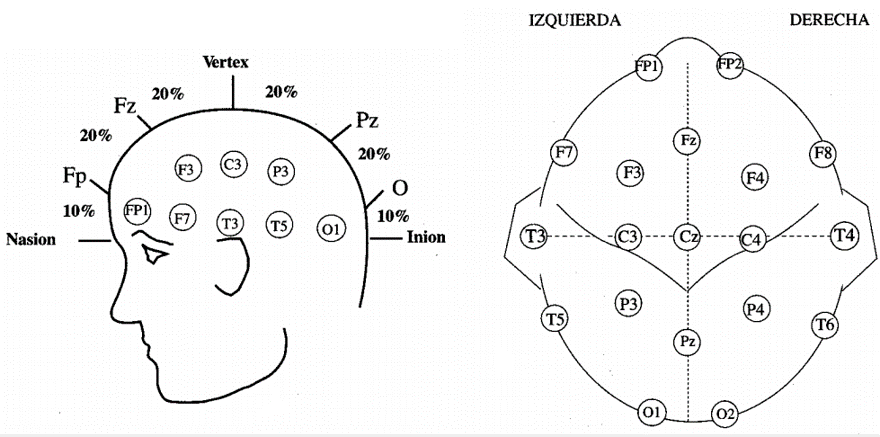
\includegraphics[scale=0.7]{eeg0.png}
\caption{Electrodos para EEG.} 
\label{fig:eeg}
\end{center}
\end{figure}

\begin{figure}[H]
\begin{center}
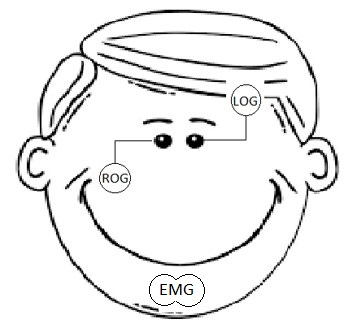
\includegraphics[scale=0.9]{cara1.jpg}
\caption{Electrodos de EOG y EMG.}
\label{fig:cara}
\end{center}
\end{figure}

Previamente a la colocaci\'on de cada electrodo, se frota la zona de inter\'es con un algod\'on empapado en crema abrasiva con el objetivo de eliminar las c\'elulas muertas y la grasa de la piel. Posteriormente, la copa de cada electrodo se rellena con una pasta electrol\'itica conductora (Ten20, Weaver) para mejorar la conductividad entre la piel y el electrodo. Los electrodos para registrar el EEG se fijar\'an al cuero cabelludo con colodi\'on (soluci\'on al 4\%, Panreac), mientras que los electrodos de poligraf\'ia (EOG y EMG) son adheridos a la piel de la cara con cinta quir\'urgica extra adhesiva (Cinta Micropore®). Para acelerar el proceso de fijaci\'on y secado del colodi\'on, se aplica aire comprimido a cada electrodo colocado sobre el cuero cabelludo. Como se muestra a continuaci\'on en la Figura \ref{fig:foto}\\

\begin{figure}[H]
\begin{center}
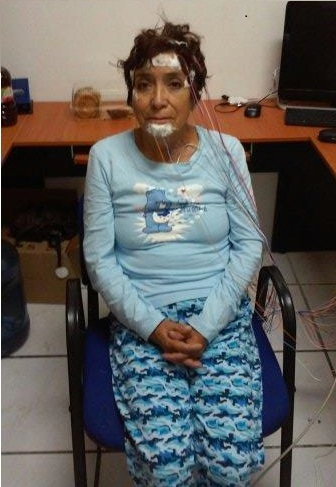
\includegraphics[scale=0.5]{v0.jpg}
\caption{Colocaci\'on de electrodos en adulto mayor para estudio PSG}
\label{fig:foto}
\end{center}
\end{figure}

Finalmente las se\~nales electrofisiol\'ogicas de cada registro PSG son amplificadas, filtradas y digitalizadas con el programa para ordenador: Registro de sue\~no, para su posterior interpretaci\'on.

\section{M\'etodo matem\'atico}

Pese a que recientemente se ha demostrado que las se\~nales biol\'ogicas son t\'ipicamente complejas y representan procesos que son no lineales y no estacionarios, las herramientas para analizar tales se\~nales a menudo siguen asumiendo la linealidad, estacionalidad y las condiciones de equilibrio. Lo que conlleva a resultados incompletos que pueden tener valor cl\'inico significativo.\\

El an\'alisis fractal es uno de los enfoques m\'as prometedores para extraer tal informaci\'on faltante de los an\'alisis lineales de las series de tiempo fisiol\'ogicas. El cu\'al se muestra a continuaci\'on \cite{Peng}. 

\subsection{Objetos fractales y proceso autosimilar}

Para definir un objeto fractal, son necesarios algunos conceptos que se enuncian a continuaci\'on:

\begin{definition}{Autosimilar}
Un espacio topologico compacto $X$ es autosimilar si existe un conjunto finito $S$ que pertenece a un conjunto de homeomorfismos no suprayectivos $\{f_s : s \in S\}$ el cual: $$X=\displaystyle \cup_{s \in S} f_s(X)$$
\end{definition}

La autosimilitud se ilustra, con un objeto que se compone de subunidades y subsubunidades en m\'ultiples niveles que se asemejan a la estructura original del objeto como en la Figura \ref{fig:ventanas}.  Sin embargo, en el mundo real, hay necesariamente l\'imites inferiores y superiores \cite{Frac}.\\

\begin{definition}{Dimensi\'on fractal}
En geometr\'ia de fractales, la dimensi\'on fractal $D$ es un n\'umero real que generaliza el concepto de dimensi\'on ordinaria para objetos geom\'etricos que no admiten espacio tangente.
\end{definition}

Existen diferentes dimensiones fractales, frecuentemente, resultan equivalentes aunque no siempre. Para el presente trabajo, la dimensi\'on fractal $D$ se calcula como: $D=3-\alpha$ \cite{Peng}. Con las dos definiciones anteriores, se define un objeto fractal.  

\begin{definition}
Un objeto fractal es un objeto geom\'etrico que tiene una dimensi\'on fractal y es autosimilar. \cite{Goldbberge}
\end{definition}

Existen diferentes figuras y objetos de fractales, que se pueden programar en alg\'un programa, pero tambi\'en se encuentran en la naturaleza, algunos de fractales se muestran en la siguiente imagen \ref{fig:fractales}.

\begin{figure}[H]
\begin{center}
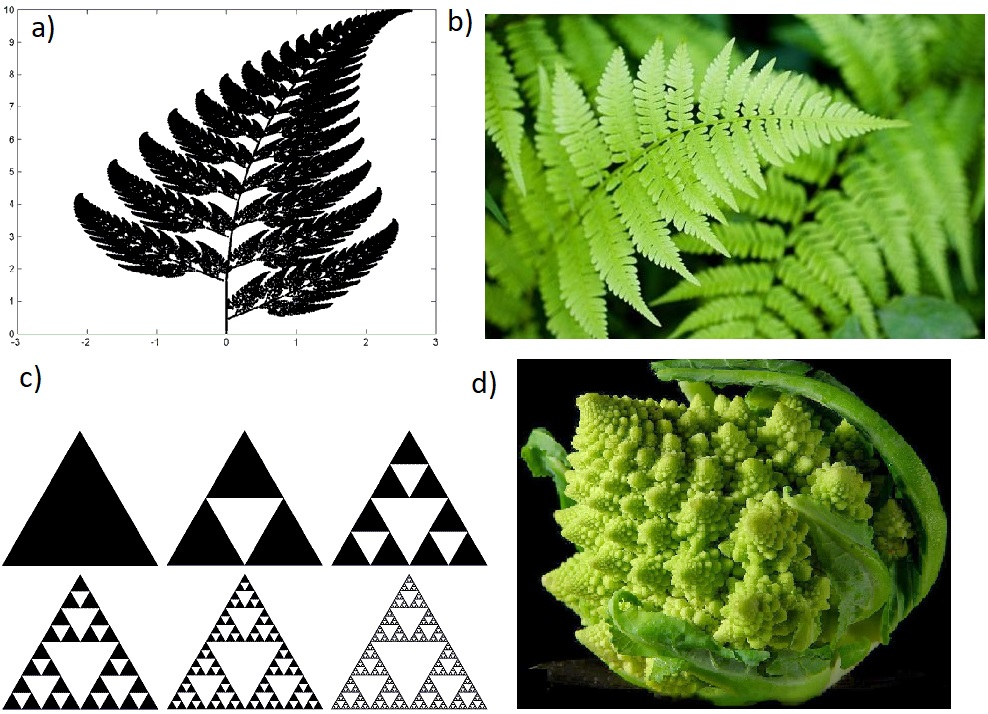
\includegraphics[scale=0.4]{fractales.jpg}
\caption{Los fractales del lado izquierda se han programado, mientras que los de la derecha se encuentran en la naturaleza. a)Helecho de Barnsley. b)Helecho. c)Tri\'angulo de Sierpinski. d)Brocoli romano.}
\label{fig:fractales}
\end{center}
\end{figure}

El concepto de fractalidad se extiende al proceso de an\'alisis de procesos temporales complejos, como son las series de tiempo. Dado que \'estas constan de dos variables f\'isicas diferentes, el tiempo y la variable que cambia con respecto al tiempo. Para determinar si una serie de tiempo es autosimilar se realiza lo siguiente:
\begin{enumerate}
\item[i)]Se considera la serie de tiempo original.
\item[ii)]Se toma un subconjunto de la misma.
\item[iii)]El subconjunto seleccionado se ajusta al tama\~no de la original.
\item[iv)]Se compara la original con la anterior.
\end{enumerate}

\begin{figure}[H]
\begin{center}
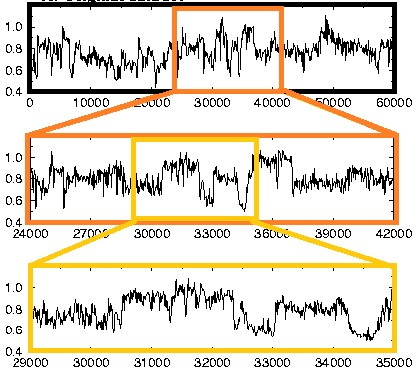
\includegraphics[scale=0.7]{ventanas.jpg}
\caption{Aqu\'i se ilustra el proceso para determinar la autosimilitud de una serie de tiempo.}
\label{fig:ventanas}
\end{center}
\end{figure}

Para comparar correctamente un subconjunto de una serie de tiempo con el conjunto de datos original, necesitamos dos factores de ampliaci\'on (los ejes horizontal y vertical), y ya que estos dos ejes representan diferentes variables f\'isicas, la serie de tiempo cumplir\'a con ser autosimilar si:
\begin{equation}
y(t)\stackrel{d}{\equiv} a^{\alpha} y\left(\frac{t}{a}\right)
\label{sim}
\end{equation}

Donde $\stackrel{d}{\equiv}$ significa que las propiedades estad\'isticas de ambos lados de la ecuaci\'on son id\'enticas. Es decir, el proceso autosimilar $y(t)$ con un par\'ametro $\alpha$ tiene la distribuci\'on de probabilidad id\'entica como un proceso correctamente reescalado $a^{\alpha} y\left(\frac{t}{a}\right)$, esto quiere decir que una serie de tiempo que ha sido reescalada sobre el eje $x$ por un factor $a\left(t\rightarrow \frac{t}{a}\right)$ y en el eje $y$ por el factor $a^{\alpha}(y\rightarrow a^{\alpha}y)$. El exponente $\alpha$ es llamado: par\'ametro de autosimilitud.\\

En la pr\'actica, sin embargo, es imposible determinar si dos procesos son estad\'isticamente id\'enticos, ya que este criterio estricto requiere que tengan funciones de distribuci\'on id\'enticas (incluyendo no solo la media y la varianza, sino tambi\'en todos los momentos superiores). Por lo que generalmente se aproxima esta igualdad con un criterio m\'as d\'ebil examinando solo las medias y las varianzas (primer y segundo momentos) de las funciones de distribuci\'on para ambos lados de la ecuaci\'on \ref{sim}.\\

La Figura \ref{fig:prob} muestra un ejemplo de una serie de tiempo de autosimilar. N\'otese que, con la elecci\'on adecuada de los factores de escala en los ejes X e Y, la serie de tiempo se reajustar\'a (Fig.\ref{fig:prob}-(b)) y se asemejar\'a a la serie de tiempo original (Fig.
\ref{fig:prob}-(a)). 

\begin{figure}[H]
\begin{center}
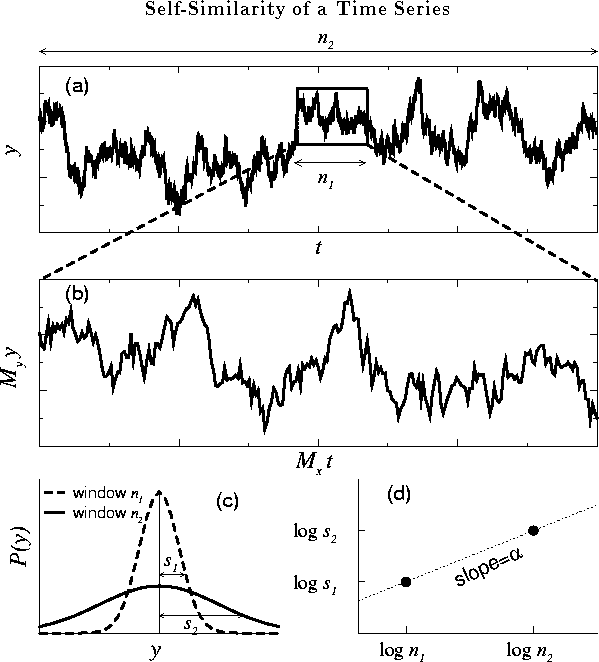
\includegraphics[scale=0.38]{prob.png}
\caption{{\bf Ilustraci\'on del concepto de la autosimilitud.} {\bf (a).} Dos ventanas de observaci\'on, con escalas de tiempo $n_1$ y $n_2$ se muestran para una serie de tiempo autosimilar de $y(t)$. {\bf (b).} Aumento de la ventana m\'as peque\~na con la escala de tiempo $n_1$. T\'engase en cuenta que las fluctuaciones en (a) y (b) tienen un aspecto similar a condici\'on de que dos factores de aumento diferentes, $M_x$ y $M_y$ se aplican a las escalas horizontales y vertical, respectivamente. {\bf (c).} La distribuci'on de probabilidad, $P(y)$, de la variable $y$ para las dos ventanas en $(\alpha)$, donde $s_1$ e $s_2$ indican las desviaciones est\'andar para estas dos funciones de distribuci\'on. {\bf (d).} Log -log de las escalas caracter\'isticas de las fluctuaciones, $s$, frente a los tama\~nos de ventana, $n$.}
\label{fig:prob}
\end{center}
\end{figure}

El par\'ametro $\alpha$ de la ecuaci\'on \ref{sim} puede ser calculado por la siguiente relaci\'on: 
\begin{equation}
\alpha= \frac{\ln{M_y}}{\ln{M_x}}
\label{alp}
\end{equation}
donde $M_x$ y $M_y$ son los factores de amplificaci\'on  del eje $x$ y eje $y$ respectivamente del subconjunto que se quiere ajustar al tama\~no de la serie de tiempo original.\\

Por lo general, en la pr\'actica no se conoce el valor del exponente $\alpha$ de antemano. En su lugar, nos enfrentamos al reto  de extraer este exponente de escala (si existe) a partir de  una serie de tiempo dado. Por lo tanto, es necesario estudiar la serie de tiempo en las ventanas de observaci\'on con diferentes tama\~nos y adoptar un criterio d\'ebil de autosimilitud definido anteriormente para calcular el exponente $\alpha$.\\

La idea b\'asica se ilustra en la Figura \ref{fig:prob}. Dos ventanas de observaci\'on (Fig \ref{fig:prob}-(a)), ventana 1 con tama\~no $n_1$ y la ventana 2 con tama\~no horizontal $n_2$, fueron seleccionados arbitrariamente para demostrar dicho procedimiento. De tal forma es f\'acil determinar el factor de aumento a lo largo de la direcci\'on horizontal, $\displaystyle M_x=\frac{n_2}{n_1}$. Pero para el factor de aumento a lo largo de la direcci\'on vertical, $M_y$, necesitamos determinar las escalas verticales, caracter\'isticas de la ventana original y la del subconjunto. Una manera de hacerlo es examinando las distribuciones de probabilidad (histogramas) de la variable y para estas dos ventanas de observaci\'on (Fig. \ref{fig:prob}-(c)).\\

Se puede definir una estimaci\'on razonable de las escalas caracte\'isticas para las alturas verticales, es decir, las fluctuaciones t\'ipicas de $y$, usando las desviaciones est\'andar de estos dos histogramas, denominadas $s_1$ y $s_2$, respectivamente. Por lo tanto, tenemos $M_y=\frac{s_2}{s_1}$. Sustituyendo $M_x$ y $M_y$ en la ecuaci\'on \ref{alp}, obtenemos:
\begin{equation}
\alpha=\frac{\ln{M_y}}{\ln{M_x}}=\frac{\ln {\displaystyle \bigg(\frac{s_2}{s_1} \bigg)}}{\ln {\displaystyle \bigg(\frac{n_2}{n_1} \bigg)}}=\frac{\ln{s_2} - \ln{s_1}}{\ln{n_2} - \ln{n_1}}
\label{alp1}
\end{equation}

La relaci\'on de la ecuaci\'on \ref{alp1} es simplemente la pendiente de la l\'inea que une a los puntos $(n_1,s_1)$ y $(n_2,s_2)$ en la gr\'afica \textit{$\log-\log$}. Es decir que  el exponente $\alpha$ se calcula ajustando una l\'inea en el gr\'afico \textit{$\log-\log$} de $s$ versus $n$ a trav\'es del rango pertinente de escalas.

\subsection{An\'alisis de fluctuaciones sin tendencia (DFA)}

Sin embargo, el proceso anterior para calcular el par\'ametro de autosimilitud $\alpha$ solo es aplicable para series de tiempo estacionarias, es decir, aquellas con media, desviaci\'on est\'andar y momentos estad\'isticos superiores, as\'i como funciones de correlaci\'on invariantes con el paso del tiempo. No obstante las series de tiempo fisiol\'ogicas a analizar son en gran medida no estacionarias.\\

Uno de los recursos para obtener el par\'ametro de autosimilitud de series de tiempo no estacionarias es el a\'alisis de flutuaci\'on sin tendencia o DFA (\textit{Detrended Fluctuation Analysis}, por sus siglas en ingl\'es) \cite{Peng}, no es m\'as que una ra\'iz cuadrada modificada, usada para determinar de forma m\'as evidente el proceso autosimilar de integraci\'on. %Este m�todo se ha aplicado con �xito en una amplia variedad de series de tiempo, simuladas o fisiol�gicas en los �ltimos a�os (Peng y cols., 1994 y 1995; Buldyrev y cols., 1993; Ossadnik y cols., 1994; Hausdorff y cols., 1995; Hausdorff y cols., 1996; Rodr�guez y cols., 2011) 
El cual se describe a continuaci\'on:\\

Dada una serie de tiempo $x(i)$, para $i=1,2,...,N$, se integran los valores de esta serie de datos, obteniendo una nueva serie de tiempo de la siguiente forma: 
\begin{equation}
\displaystyle y(k)=\sum_{i=1}^{k}(x(i)-\hat{x}) \label{st_integrada}
\end{equation}
donde $\displaystyle \hat{x}=\frac{1}{N} \sum_{i=1}^N x(i)$, es decir el valor promedio de $x$. Donde la ecuaci\'on \eqref{st_integrada} mapea la serie de tiempo a un proceso autosimilar.\\

Una vez obtenido el mapeo se mide la escala vertical de caracter\'isticas de la serie de tiempo integrada, lo cual se obtiene dividiendo a $y(k)$ en ventanas de igual tama\~no $n$. Donde para cada una de las ventadas de datos se calcula el ajuste lineal de m\'inimos cuadrados o bien la tendencia local de la ventana correspondiente.\\

%Revisar--------------
El valor de la coordenada $y$ de la l\'inea recta se denota por $y_n(k)$. Para eliminar la tendencia de $y(k)$ para cada ventana, se sustrae la tendencia local lineal $y_n(k)$. Para cada tama\~no de ventana $n$, la escala caracter\'istica para las fluctuaciones en la serie integrada y sin tendencia es dada por:
\begin{equation}
F(n)=\sqrt{\frac{1}{N}\sum_{i=1}^{N}(y(i)-y_n(k))^2} \label{Sin_Tendencia}
\end{equation}
Siendo F un valor similar a la desviaci\'on est\'andar, sin embargo, no id\'entica.\\

Este c\'alculo se repite en todas las escalas de tiempo (tama\~nos de ventanas. Figura \ref{fig:DFA2}) para proporcionar una relaci\'on entre $F(n)$ y la ventana de tama\~no $n$. T\'ipicamente $F(n)$ se incrementar\'a con el tama\~no $n$ de ventana.\\

\begin{figure}[h]
\begin{center}
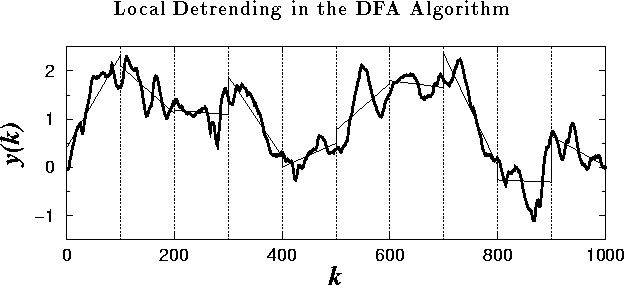
\includegraphics[scale=0.5]{DFA2.png}
\caption{{\bf Serie de tiempo integrada:} $\displaystyle y(k)=\sum_{i=1}^{k}(x(i)-\hat{x})$ donde $x(i)$ es el intervalo de latidos, las l\'ineas de puntos verticales indican cajas de tama\~no $n=100$ y los segmentos de l\'inea rectos s\'olidos representan la tendencia calculada en cada caja por un ajuste lineal de m\'inimos cuadrados(\cite{Goldberger}}
\label{fig:DFA2}
\end{center}
\end{figure}

Una relaci\'on lineal en un gr\'afico de doble logaritmo ($\log n$ vs $\log F(n)$) indica la presencia de escalamiento (autosimilitud). Es decir, las fluctuaciones en ventanas peque\~nas est\'an relacionadas con las fluctuaciones de las ventanas m\'as grandes, siguiendo una forma de ley de potencia. La l\'inea en relaci\'on $\log n$ y $\log F(n)$ determinar\'a el exponente de escalamiento (representar\'a las fluctuaciones determinadas por la ecuaci\'on \eqref{Sin_Tendencia}) o par\'ametro de autosimilitud $\alpha$, esto es: 
\begin{equation}
F(n)=n^{\alpha}
\end{equation}
 
El DFA ha revelado la correlaci\'on de largo alcance en series de tiempo aparentemente irregulares \cite{Peng} de la siguiente manera:
\begin{itemize}
\item $0<\alpha<0.5$ Presenta anticorrelaci\'on.
\item $\alpha\simeq0.5$ Ruido blanco.
\item $\alpha>0.5$ Indica la presencia de una correlaci\'on de largo alcance. 
\item $\alpha\simeq1$ Corresponde la ruido rosa.
\item $\alpha\simeq1.5$ Ruido caf\'e.
\end{itemize}

Siendo el DFA un m\'etodo para detectar escalas observadas, es decir, la correlaci\'on de largo alcance en la serie de tiempo no estacionarias. Lo cual se ilustra en el siguiente ejemplo. 

-----------------------------%eEjemplo%---------------------------------------------------

\subsubsection{Ejemplo en \'epoca de sue\~no MOR}

Para tener una ida m\'as clara de lo que se esta realizando con el m\'etodo DFA, se considera una \'epoca de sue\~no MOR cualquiera, la cual consta de 30 segundos, con una frecuencia de 512 Hz, teniendo un total de 15,360 puntos. Representados en el siguiente gr\'afico \ref{ejemplo}.  

\begin{figure}[H]
\begin{center}
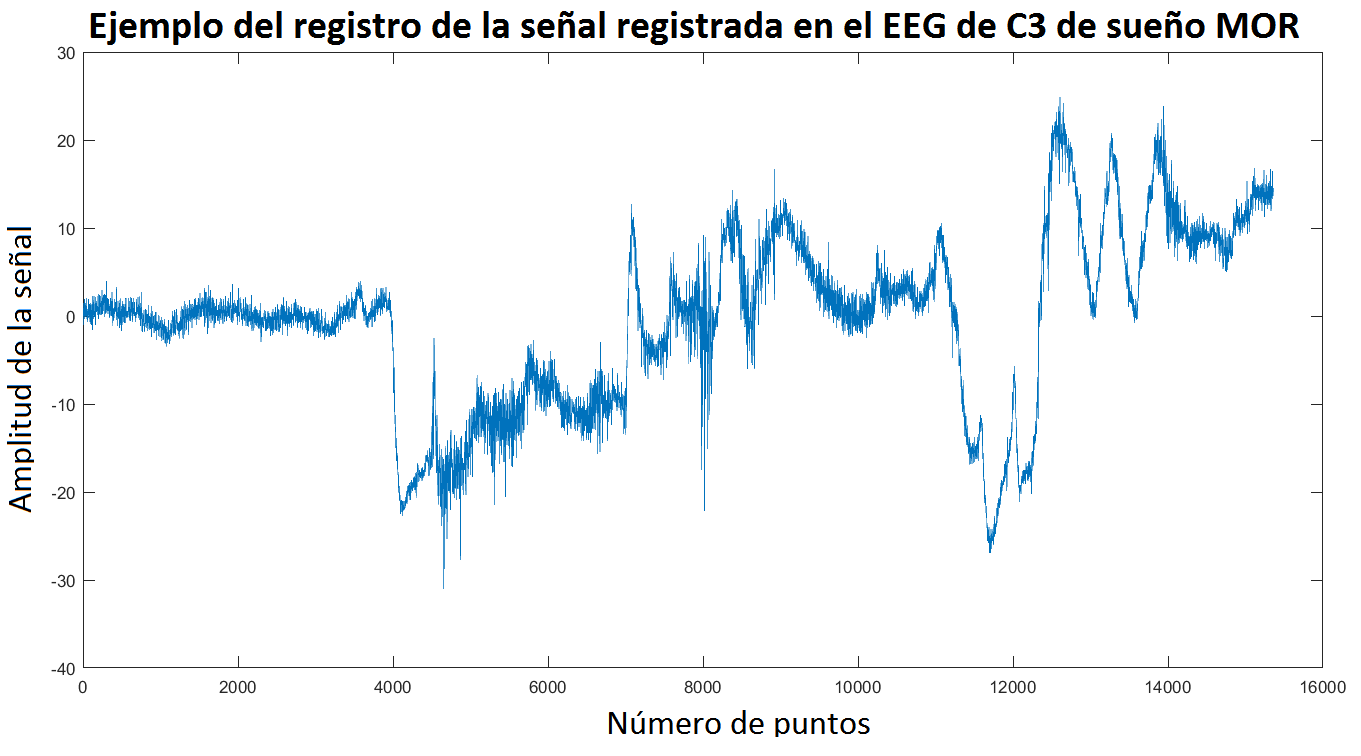
\includegraphics[scale=0.3]{Ejemplo.png}
\caption{Gr\'afico de los datos obtenidos del canal C3 en la \'epoca de sue\~no MOR de un adulto mayor sin deterioro cognitivo.}
\label{ejemplo}
\end{center}
\end{figure}

Primero es necesario saber el tama\~no que tendr\'an las ventanas que dividir\'an a la serie original, en este caso vamos a considerar que el tama\~no de ventana sea de 3350 puntos, teniendo un total de 4 ventanas, es decir, 13,400 puntos en total. Notemos que no se estan considerando todos los puntos de la serie original, ya que en caso de considerar una quinta ventana, esta no estar\'ia completa.\\

Sea a serie de tiempo $x(i)=1,2,3,...,13400$, calculamos el promedio de los 13400 puntos y se tiene $\displaystyle \hat{x}=\frac{1}{13400} \sum_{i=1}^{13400} x(i)=-2.0891$. Calculamos la nueva serie de tiempo $y(k)$ \eqref{st_integrada}.\\

\begin{table}[]
\centering
\caption{Ecuaciones para obtener la serie $y(k)$}
\begin{tiny}
\begin{tabular}{ll}
\hline
$k$      & $y(k)$                                                                                \\
\hline
1        & $\displaystyle y(1)=\sum_{i=1}^{1}(x(i)-(-2.0891))=0.9-(-2.0891)=2.9891$                            \\
2        & $\displaystyle y(2)=\sum_{i=1}^{2}(x(i)-(-2.0891))=y(1)+(-0.4+(-2.0891))=4.6782$                    \\
3        & $\displaystyle y(3)=\sum_{i=1}^{3}(x(i)-(-2.0891))=y(2)+(-1+(-2.0891))=5.7673$                      \\
$\vdots$ & \multicolumn{1}{c}{$\vdots$}                                                          \\
13400    & $\displaystyle y(13400)=\sum_{i=1}^{13400}(x(i)-(-2.0891))
=y(13399)+(9.2+(-2.0891))=0.000000000454$\\
\hline
\end{tabular}
\end{tiny}
\label{tabla}
\end{table}

Una vez que se obtienen los puntos de $y(k)$, se puede apreciar en el siguiente gr\'afico \ref{ejemplo1}:

\begin{figure}[H]
\begin{center}
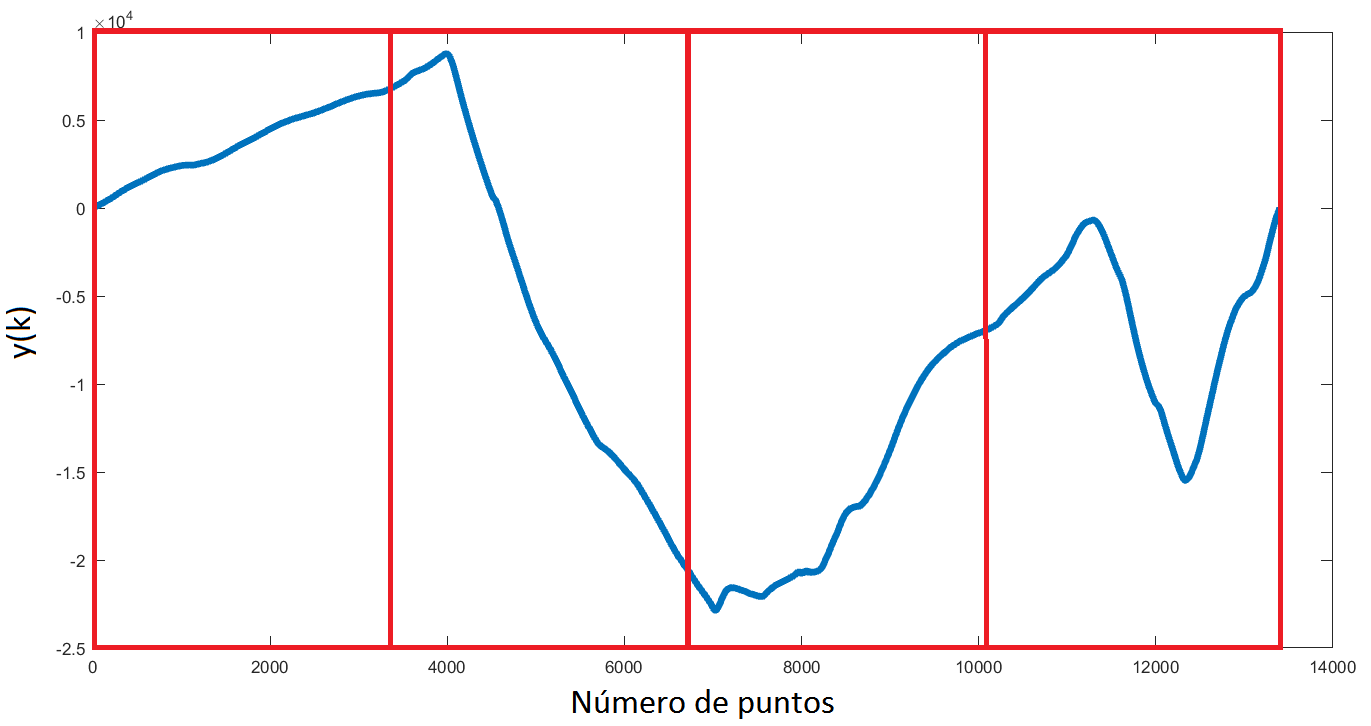
\includegraphics[scale=0.35]{ejemplointegrada1.png}
%Falta agrergar las lineas obtenidas por minimos cuadrados.
\caption{Representaci\'on de la separaci\'on de las ventanas de tama\~no 3350 de la serie intgrada $y(k)$. \ref{ejemplo}}
\label{ejemplo1}
\end{center}
\end{figure}

Para quitar la tendencia lineal local de cada ventana se realiza un ajuste lineal por m\'inimos cuadrados.\\ 

Se denota al valor de la coordenada $y$ de la l\'inea recta como $y_{4}(k)$. Para quitar la tendencia lineal de $y(k)$ se sustrae la tendencia local lineal $y_{4}(k)$. De lo anterior se tiene:

\begin{equation*}
\begin{split}
F(3350) & =\sqrt{\frac{1}{13400}\sum_{i=1}^{13400}(y(i)-y_4(k))^2}\\
& \quad =\sqrt{4813494,01815568}\\
& \quad =2193,96764291447
\end{split}
\end{equation*}



Este paso se repite para ventanas de 6 puntos hasta 9494 puntos. Una vez que tenemos tales resultados, procedemos a registrarlos en un tabla, para posteriormente realizar la escala logar\'itmica del tama\~no de la ventana con respecto a la fluctuaci\'on que se obtuvo \ref{tablalog}.

\begin{table}[H]
\centering
\caption{Datos obtenidos del tama\~no de las ventanas y la fluctuaci\'on correspondiente. As\'i como su escala logar\'itmica}
\label{tablalog}
\begin{tiny}
\resizebox{\textwidth}{!}{%
\begin{tabular}{|
>{\columncolor[HTML]{FFFFC7}}l |l|l|l|
>{\columncolor[HTML]{FFFFC7}}l |l|l|l|}
\hline
\multicolumn{1}{|c|}{\cellcolor[HTML]{FFCE93}n} & \multicolumn{1}{c|}{\cellcolor[HTML]{FFCE93}Fn} & \multicolumn{1}{c|}{\cellcolor[HTML]{FFCE93}log(n)} & \multicolumn{1}{c|}{\cellcolor[HTML]{FFCE93}log(Fn)} & \multicolumn{1}{c|}{\cellcolor[HTML]{FFCE93}n} & \multicolumn{1}{c|}{\cellcolor[HTML]{FFCE93}Fn} & \multicolumn{1}{c|}{\cellcolor[HTML]{FFCE93}log(n)} & \multicolumn{1}{c|}{\cellcolor[HTML]{FFCE93}log(Fn)} \\ \hline
6 & 0,3410 & 0,7782 & -0,4673 & 272 & 32,7163 & 2,4346 & 1,5148 \\ \hline
7 & 0,4688 & 0,8451 & -0,3290 & 296 & 44,7784 & 2,4713 & 1,6511 \\ \hline
8 & 0,5954 & 0,9031 & -0,2252 & 323 & 43,3917 & 2,5092 & 1,6374 \\ \hline
9 & 0,7126 & 0,9542 & -0,1471 & 352 & 52,8627 & 2,5465 & 1,7231 \\ \hline
10 & 0,8153 & 1,0000 & -0,0887 & 384 & 70,8892 & 2,5843 & 1,8506 \\ \hline
11 & 0,9014 & 1,0414 & -0,0451 & 419 & 74,4249 & 2,6222 & 1,8717 \\ \hline
12 & 1,0333 & 1,0792 & 0,0142 & 457 & 97,3706 & 2,6599 & 1,9884 \\ \hline
13 & 1,1791 & 1,1139 & 0,0716 & 498 & 102,1631 & 2,6972 & 2,0093 \\ \hline
14 & 1,2940 & 1,1461 & 0,1119 & 543 & 143,0328 & 2,7348 & 2,1554 \\ \hline
16 & 1,4535 & 1,2041 & 0,1624 & 592 & 153,4498 & 2,7723 & 2,1860 \\ \hline
17 & 1,5668 & 1,2304 & 0,1950 & 645 & 183,7535 & 2,8096 & 2,2642 \\ \hline
19 & 1,7972 & 1,2788 & 0,2546 & 704 & 194,0914 & 2,8476 & 2,2880 \\ \hline
20 & 1,8415 & 1,3010 & 0,2652 & 768 & 229,6352 & 2,8854 & 2,3610 \\ \hline
22 & 2,1198 & 1,3424 & 0,3263 & 838 & 273,3345 & 2,9232 & 2,4367 \\ \hline
24 & 2,3055 & 1,3802 & 0,3628 & 913 & 268,1394 & 2,9605 & 2,4284 \\ \hline
26 & 2,3492 & 1,4150 & 0,3709 & 996 & 288,2378 & 2,9983 & 2,4598 \\ \hline
29 & 2,6030 & 1,4624 & 0,4155 & 1086 & 398,2359 & 3,0358 & 2,6001 \\ \hline
31 & 2,7657 & 1,4914 & 0,4418 & 1184 & 419,9217 & 3,0734 & 2,6232 \\ \hline
34 & 2,9859 & 1,5315 & 0,4751 & 1292 & 408,4695 & 3,1113 & 2,6112 \\ \hline
37 & 3,1225 & 1,5682 & 0,4945 & 1409 & 520,8524 & 3,1489 & 2,7167 \\ \hline
40 & 3,3003 & 1,6021 & 0,5185 & 1536 & 455,9131 & 3,1864 & 2,6589 \\ \hline
44 & 3,5138 & 1,6435 & 0,5458 & 1675 & 726,4486 & 3,2240 & 2,8612 \\ \hline
48 & 3,7020 & 1,6812 & 0,5684 & 1827 & 971,6796 & 3,2617 & 2,9875 \\ \hline
52 & 3,8923 & 1,7160 & 0,5902 & 1992 & 828,6775 & 3,2993 & 2,9184 \\ \hline
57 & 4,2202 & 1,7559 & 0,6253 & 2172 & 1194,7214 & 3,3369 & 3,0773 \\ \hline
62 & 4,0091 & 1,7924 & 0,6030 & 2369 & 1053,5310 & 3,3746 & 3,0226 \\ \hline
68 & 4,8110 & 1,8325 & 0,6822 & 2583 & 1625,1189 & 3,4121 & 3,2109 \\ \hline
74 & 4,9322 & 1,8692 & 0,6930 & 2817 & 1252,1294 & 3,4498 & 3,0976 \\ \hline
81 & 5,6484 & 1,9085 & 0,7519 & 3072 & 1237,9050 & 3,4874 & 3,0927 \\ \hline
88 & 6,1113 & 1,9445 & 0,7861 & {\color[HTML]{FE0000} 3350} & {\color[HTML]{FE0000} 2193,9676} & {\color[HTML]{FE0000} 3,5250} & {\color[HTML]{FE0000} 3,3412} \\ \hline
96 & 5,8498 & 1,9823 & 0,7671 & 3653 & 1501,8246 & 3,5626 & 3,1766 \\ \hline
105 & 7,3770 & 2,0212 & 0,8679 & 3864 & 629,9272 & 3,5870 & 2,7993 \\ \hline
114 & 7,8249 & 2,0569 & 0,8935 & 4344 & 1846,5948 & 3,6379 & 3,2664 \\ \hline
124 & 9,5595 & 2,0934 & 0,9804 & 4708 & 2651,8729 & 3,6728 & 3,4236 \\ \hline
136 & 10,2739 & 2,1335 & 1,0117 & 5166 & 1838,2147 & 3,7132 & 3,2644 \\ \hline
148 & 10,8933 & 2,1703 & 1,0372 & 5634 & 2236,2678 & 3,7508 & 3,3495 \\ \hline
161 & 13,5273 & 2,2068 & 1,1312 & 6144 & 3190,2805 & 3,7885 & 3,5038 \\ \hline
176 & 13,7475 & 2,2455 & 1,1382 & 6700 & 2993,9076 & 3,8261 & 3,4762 \\ \hline
191 & 16,9589 & 2,2810 & 1,2294 & 7306 & 3947,2793 & 3,8637 & 3,5963 \\ \hline
209 & 23,1499 & 2,3201 & 1,3645 & 7968 & 3414,3127 & 3,9013 & 3,5333 \\ \hline
228 & 22,4216 & 2,3579 & 1,3507 & 8689 & 4691,7909 & 3,9390 & 3,6713 \\ \hline
249 & 34,2265 & 2,3962 & 1,5344 & 9474 & 6141,7400 & 3,9765 & 3,7883 \\ \hline
\end{tabular}%
}
\end{tiny}
\end{table}

Una vez obtenidos los valores de la variable dependiente $Fn$ dado el tama\~no de la ventana $n$, los valores se representan con una doble escala logar\'itmica ($\log Fn$,$\log n$), como se muestran en la figura \ref{ejem1}.

\begin{figure}[H]
\begin{center}
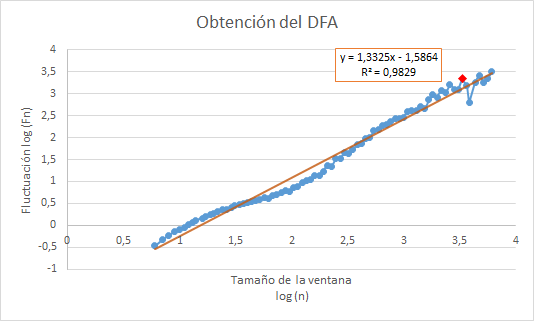
\includegraphics[scale=1]{ejem2.png}
\caption{Representaci\'on de la doble escala logar\'itmica $\log Fn$ vs $\log n$, representada de color azul, donde se resalta de color rojo al tama\~no de ventana 3350, el cual ayudo para ilustrar el m\'etodo DFA. Mostrando a su vez la l\'inea de tendencia correspondiente al mismo, de color naranja, as\'i como la ecuaci\'on de la misma, para poder apreciar el valor de su pendiente, es decir, el par\'ametro de autosimilitud $\alpha$.}
\label{ejem1}
\end{center}
\end{figure}

Posteriormente, se obtiene la l\'inea de tendencia de tal grafico, cuya ecuaci\'n nos permite conocer el par\'ametro de autosimilitud $\alpha$, siendo $\alpha$ representado como la pendiente de la misma.\\

De esta manera de obtiene el valor de autosimilud de una \'epoca de sue\~no MOR, el cual posteriormente se compara con los valores de autocorrelaci\'on establecidos en el la secci\'on del An\'alisis de Fluctuaci\'on sin Tendencia (DFA). En este caso el valor es 1.256, acercandose al par\'ametro $\alpha=1$, ruido rosa. 

\subsection{Relaci\'on interhemisf\'erica}

Cuando una persona esta despierta la relaci\'on que existe entre el hemisferio derecho y el izquierdo es baja, sin embargo, durante el sue\~o existe una mayor relaci\'on interhemisf\'erica. Por lo que tambi\'en se considero un tema de inter\'es, el analizar el color del ruido en el sue\~no MOR considerando la interacci\'on de ambos hemisferios, as\'i como la relaci\'on de los movimientos oculares (LOG-ROG), lo cual se ilustra en la figura \ref{fig:rel}:

\begin{figure}[H]
\centering
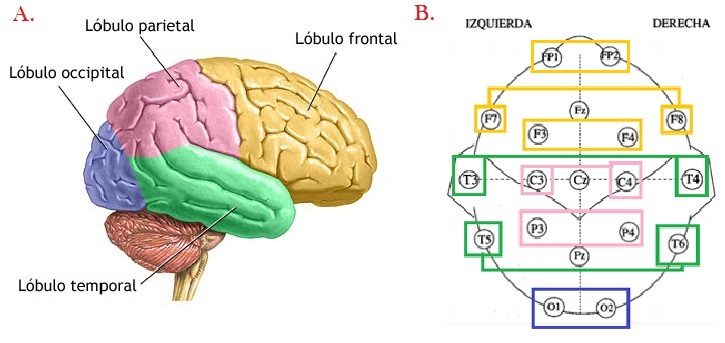
\includegraphics[scale=0.7]{rel.jpg}
\caption{{\bf A.} Partes de la corteza cerebral registradas por la polisomnograf\'ia. {\bf B.} Relaci\'on interhemisf\'erica que se desea analizar en los distintos canales registrados: FP1-FP2, F7-F8, F3-F4; T3-T4, T5-T6; C3-C4, P3-P4 y O1-O2}
\label{fig:rel}
\end{figure}


\subsection{An\'alisis de fluctuaciones sin tendencia multicanal (mDFA)} 

Tanto el estudio de Telesca y colaboradores (2007) como en el de Rosas y colaboradores (2002), el DFA se aplic\'o para 2 dimensiones de series de tiempo, y en los que se sugiere que es posible describir una f\'ormula para series de tiempo multidiemensionales (Tesis Doctoral Erika E. Rodr\'iguez Torres), es decir una generalizaci\'on del DFA.\\

El cual comienza con series de tiempo $\overrightarrow{x}(i)=(x(i)_1,x(i)_2,...,x(i)_m)$ es un $m$-vector dimensional, donde $m$ es el n\'umero de entradas o canales del registro. El DFA multicanal (mDFA)\cite{mDFA} puede ser implementado considerando los valores integrados de las series de tiempo de la ecuaci\'on \eqref{st_integrada}, esto es:
\begin{equation}
y(k)=\sum_{i=1}^{N}(\overrightarrow{x}(i)-\widehat{x})\label{stm_integrada}
\end{equation}
donde $\widehat{x}=\frac{1}{N}\sum_{i=1}^{N}\overrightarrow{x}(i)$ es el vector cuyos componentes son los promedios de las componentes de los vectores $\overrightarrow{x}(1),\overrightarrow{x}(2),...,\overrightarrow{x}(N)$ y como en la ecuaci\'on \eqref{st_integrada}, se tiene un proceso autosimilar en la ecuaci\'on \eqref{stm_integrada}.\\

A continuaci\'on se mide la escala vertical de caracter\'isticas de la serie de tiempo integrada, lo cual se obtiene dividiendo a $y(k)$ (ecuaci\'on \eqref{stm_integrada}) en ventanas de igual tama\~no $n$. Donde para cada una de las ventadas de datos se calcula el ajuste lineal de m\'inimos cuadrados o bien la tendencia local de la ventana correspondiente.\\

El vector de valores de la coordenada $y$ de la l\'inea recta se denota por $\overrightarrow{y_n}(k)$. Para eliminar la tendencia de $y(k)$ se elimina la tendencia componente por componente, as\'i  que se sustrae $\overrightarrow{y_n}(k)$. Modificando la ecuaci\'on \eqref{Sin_Tendencia} de tal manera que las contribuciones individuales de cada fluctuaci\'on sin tendencia de cada componente del vector $i=1,2,...,m$ se toma en cuenta y se define:
\begin{equation}
F(n)=\sqrt{\frac{1}{N}\sum_{i=1}^{N}\Vert y(i)-y_n(k)\Vert ^2}\label{mSin_Tendencia}
\end{equation}

Graficando los valores de $\log n$ y $\log F(n)$, se obtiene una relaci\'on lineal que indica la presencia de una ley de potencia, es decir:
\begin{equation}
F(n)=n^\alpha
\end{equation}

Donde el exponente escalar $\alpha$, o exponente de Hurst, representa las fluctuaciones de la se\~nal y se puede aproximar como la pendiente de la l\'inea relacionada $\log n$ y $\log F(n)$ como en el caso del DFA cl\'asico los diferentes valores de $\alpha$ indican las correlaciones de la serie de tiempo.\\

La contribuci\'on del mDFA se encuentra en que \'este toma en cuenta los potenciales sincronizados intersegmentales, mientras que el DFA solo considera las correlaciones de largo alcance de un solo segmento. 

%----------------------------

\section{Relaci\'on con otros m\'etodos}

En el caso de las autocorrelaciones de decaimiento de la ley de potencia, la funci\'on de correlaci\'on deca\'e con el exponente $\gamma:C(L)\sim L^{\gamma}$. Adem\'as el espectro de potencia $P(f)\sim f^{-\beta}$. Los tres exponentes est\'an relacionados por:
\begin{itemize}
\item $\gamma=2-2\alpha$
\item $\beta=2\alpha-1$
\item $\gamma=1-\beta$
\end{itemize}
Las relaciones se pueden derivar usando el teorema de Wiener-Khinchin. As\'i $\alpha$ esta ligado a la pendiente del espectro de potencia $\beta$ y es usado para describir el color del ruido por la relaci\'on $\alpha=\frac{(\beta+1)}{2}$.\\

Para el ruido Gaussiano fraccionario (FGN), tenemos $\beta\in[-1,1]$ y as\'i $\alpha=[1,0]$ y $\beta=2H-1$ donde $H$ es el exponente de Hurst  $\alpha$ para FGN es igual a $H$.\\

Para el movimiento browniano fraccional $FBM$, se tiene $\beta\in[1,3]$ y as\'i $\alpha=[1,2]$ y $\beta=2H+1$ donde $H$ es el exponente de Hurst $\alpha$ para FBM es igual a $H+1$. En este contexto, FBM es la suma acumulada o la integral de FGN, por lo tanto, los exponentes de sus espectros de potencia difieren en 2.
%-----------------------



%Resultados----------------------------------------------
\newpage
\chapter{Resultados}

\section{Preliminares}

Para el presente trabajo se cont\'o con la colaboraci\'on de 5 adultos mayores con deterioro cognitivo y 5 sin deterioro. Una vez obtenidos los datos de DFA y mDFA de cada uno, se requiere de la estad\'istica para determinar, si hay una relaci\'on entre los EEGs y el color del ruido, ya sea: blanco, rosa o caf\'e; adem\'as de resaltar las diferencias en cada canal obtenido a trav\'es de la polisomnograf\'ia. Para lo cual necesitaremos de lo siguiente:

\subsubsection{Prueba de hip\'otesis}

La prueba de hi\'otesis es un procedimiento estad\'istico que permite aceptar o rechazar una afirmaci\'on hecha con respecto a un fen\'omeno o suceso. La prueba de hip\'otesis consta de dos componentes principales: hip\'otesis nula $H_0$ e hip\'otesis alternativa $H_1$.\\

La \textbf{hip\'otesis nula $H_0$} es una afirmaci\'on sobre un par\'ametro de la poblaci\'on, por lo general incluye un no en su enunciado \cite{Estec}, mientras que la \textbf{hip\'otesis alternativa $H_1$} es la que corresponde a nuestra pregunta, es decir, la que se establece a la evidencia que se tiene.\\

Si se quiere probar que la media de una poblaci\'on es igual a $\mu_0$, entonces la prueba nula se puede expresar como: $H_0: \mu=\mu_0$. As\'i como se tiene que plantear una hip\'otesis alternativa $H_1$, si la alternativa es que la media poblacional es mayor que $\mu_0$, esta se denomina \bf{prueba de una cola}, es decir, si $H_1: \mu > \mu_0 $ (o bien $\mu < \mu_0$), y si $H_1: \mu \neq \mu_0$ se dice que es \bf{prueba de dos colas}. 

\begin{definition}
Una \textbf{prueba de hip\'otesis} es una regla para decidir si se acepta la hi\'otesis nula o se rechaza en favor de la hip\'otesis alternativa.
\end{definition}

Al tomar una decisi\'on de este tipo se corre el riesgo de cometer errores. Al rechazo de la hip\'otesis nula cuando \'esta es verdadera se le conoce como \textbf{error tipo I} y a la probabilidad de cometer este primer tipo de error se le denota $\gamma$. En cambio, a la aceptaci\'on de la hip\'otesis nula cuando \'esta es falsa recibe el nombre de \textbf{error tipo II}, y a la probabilidad de cometer este segundo tipo de error se le denota por la letra $\beta$. Las definiciones anteriores se ilustran en la siguiente tabla.\cite{Rincon}

\begin{table}[H]
\centering
%\caption{My caption}
\begin{tabular}{l|c|c|}
\cline{2-3}
 & \cellcolor[HTML]{CBCEFB}$H_0$ cierta & \cellcolor[HTML]{CBCEFB}$H_0$ falsa \\ \hline
\multicolumn{1}{|l|}{\cellcolor[HTML]{CBCEFB}Rechazar $H_0$} & \begin{tabular}[c]{@{}c@{}}Error tipo II \\ con probabilidad $\gamma$ \end{tabular} & Decisi\'on correcta \\ \hline
\multicolumn{1}{|l|}{\cellcolor[HTML]{CBCEFB}No rechazar $H_0$} & Decisi\'on correcta & \begin{tabular}[c]{@{}c@{}}Error tipo II \\ con probabilidad $\beta$ \end{tabular} \\ \hline
\end{tabular}
\label{errores}
\end{table}

\subsubsection{Prueba $t$ de Student}

La prueba $t$ de Student es una distribuci\'on de probabilidad que surge del problema de estimar lamedia de una poblaci\'on normalmente distribuida cuando el tama\~no de la muestra es peque\~no.\\

Supongamos que $Y_1,Y_2,...,Y_n$ denotan una muestra aleatoria de tama\~no $n$ de una distribuci\'on normal con media $\mu$ desconocida y varianza $\sigma^2$ desconocida. Si $\overline{Y}$ y $S$ denotan la media muestral y la desviaci\'on muestral est\'andar, respectivamente, y si $H_0: \mu = \mu_0$  es verdadera, entonces:
$$T=\frac{\overline{Y}-\mu_0}{S/\sqrt{n}}$$
tiene distribuci\'on $t$ con $n-1$ grados de libertad.\\

Como la distribuci\'on $t$ es sim\'etrica y en forma de campana, la regi\'on de rechazo para una prueba de la hip\'otesis $H_0:\mu = \mu_0$ con muestras peque\~nas debe estar localizada en las colas de la distribuci\'on $t$. La regi\'on de rechazo adecuada para la alternativa de cola superior se muestra a continuaci\'on:

\[H_1:
 \left \{
   \begin{array}{rcl}
   \mu>\mu_0 \hspace{1cm} \text{(alternativa de cola superior)}\\
   \mu<\mu_0 \hspace{1cm} \text{(alternativa de cola inferior)}\\
\mu\neq\mu_0 \hspace{1cm} \text{(alternativa de dos colas)}
    \end{array}
\right. \]
       
\[\text{Regi\'on de rechazo:}
 \left \{
   \begin{array}{rcl}
      t>t_\gamma \hspace{1cm} \text{(regi\'on de rechazo de cola superior)}\\
      t<t_\gamma \hspace{1cm} \text{(regi\'on de rechazo de cola inferior)}\\
|t|>t_{\gamma/2} \hspace{1cm} \text{(regi\'on de rechazo de dos colas)}
   \end{array}
\right. \]

\cite{Est}

\section{Color del ruido de cada canal}

Como se menciono en el cap\'itulo 4 los registros obtenidos de la polisomnograf\'ia practicada a 
adultos mayores, se les identific\'o el nivel cognitivo de atenci\'on y memoria de acuerdo a los 
resultados obtenidos en los examenes Neuropsi y Mini Mental State Examination (MMSE),  para 
posteriormente hacer una distinci\'on entre los adultos con y sin deterioro cognitivo \cite{Genesis}.\\

Cada señal esta compuesta por 22 canales en total, ya que la se\~nal es una noche de sue\~no, para 
este trabajo solo se consideran las \'epocas de sue\~no MOR, donde cada \'epoca consta de 30 
segundos, con una frecuencia de 512 Hz, es decir, 512 fluctuaciones por segundo, teniendo un total de 
15,360 datos por \'epoca. Un ejemplo de las se\~nales de la polisomnograf\'ia de cada canal, se 
ilustran en las figuras \ref{fig:reg_sano} y \ref{fig:reg_dc}, siendo la primera, una \'epoca de 
sue\~no MOR de un adulto mayor sin deterioro cognitivo y la segunda uno con deterioro cognitivo. 

\begin{figure}[H]
\centering
\includegraphics[scale=1]{senal_sin.jpg}
\caption{Señales de una \'epoca de sue\~no MOR en un adulto mayor sin deterioro cognitivo. Adaptado de \cite{Genesis}.}
\label{fig:reg_sano}
\end{figure}

\begin{figure}[H]
\centering
\includegraphics[scale=1]{senal_con.jpg}
\caption{Señales de una \'epoca de sue\~no MOR en un adulto mayor con deterioro cognitivo. Adaptado de \cite{Genesis}.}
\label{fig:reg_dc}
\end{figure}

En la Figura \ref{fig:c1_1} se muestran los resultados obtenidos del an\'alisis DFA a una serie de tiempo de una \'epoca MOR de un adulto mayor con deterioro cognitivo versus un adulto mayor sano. Donde se puede apreciar como los resultados del adulto mayor con deterioro se acercan m\'as al ruido caf\'e o browniano, $\alpha\approx 1.5$ y en cambio los resultados del participante sin deterioro se mantienen m\'as cercanos al ruido rosa o ruido biol\'ogico, $\alpha\approx 1$.\\

As\'i como tambi\'en se puede observar que el canal EMG, es decir, las se\~nales producidas por la contracci\'on del m\'usculo mentoniano tienden al ruido blanco, $\alpha\approx 0.5$.\\

\begin{figure}[H]
\centering
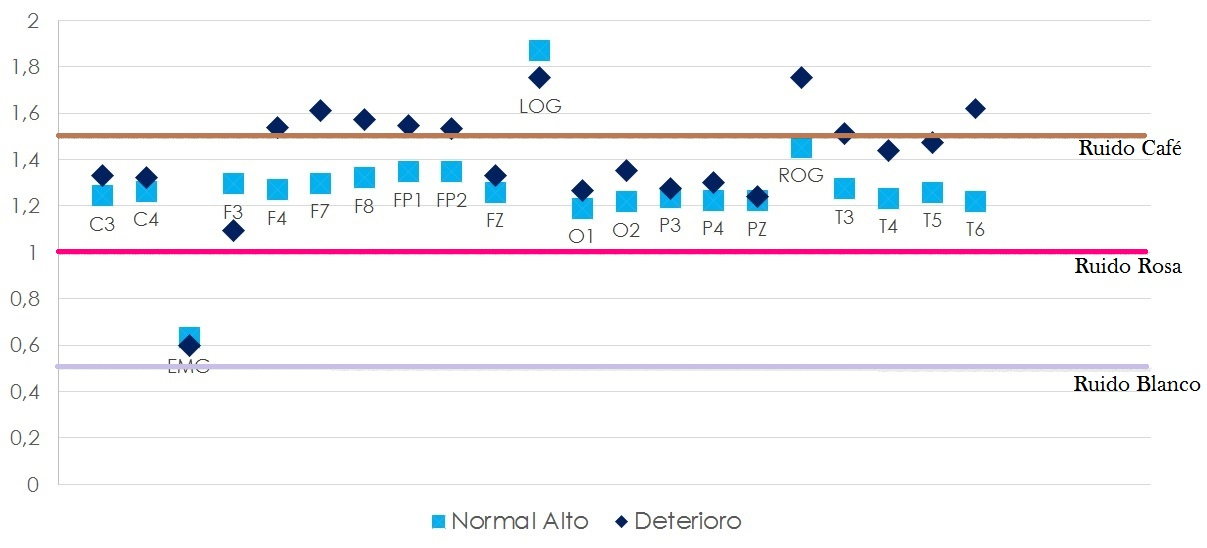
\includegraphics[scale=0.5]{comp1_1.jpg}
\caption{Aproximaci\'on del color del ruido del an\'alisis DFA de series de tiempo individuales}
\label{fig:c1_1}
\end{figure}

El an\'alisis anterior se realiz\'o para las primeras 10 \'epocas de sue\~no MOR de cada registro, para posteriormente promediar los resultados obtenidos. En la Figura \ref{fig:c1_3} se muestra la distribuci\'on de los mismos, as\'i como se puede observar que conservan la tendencia que en figura \ref{fig:c1_1}.

\begin{figure}[H]
\centering
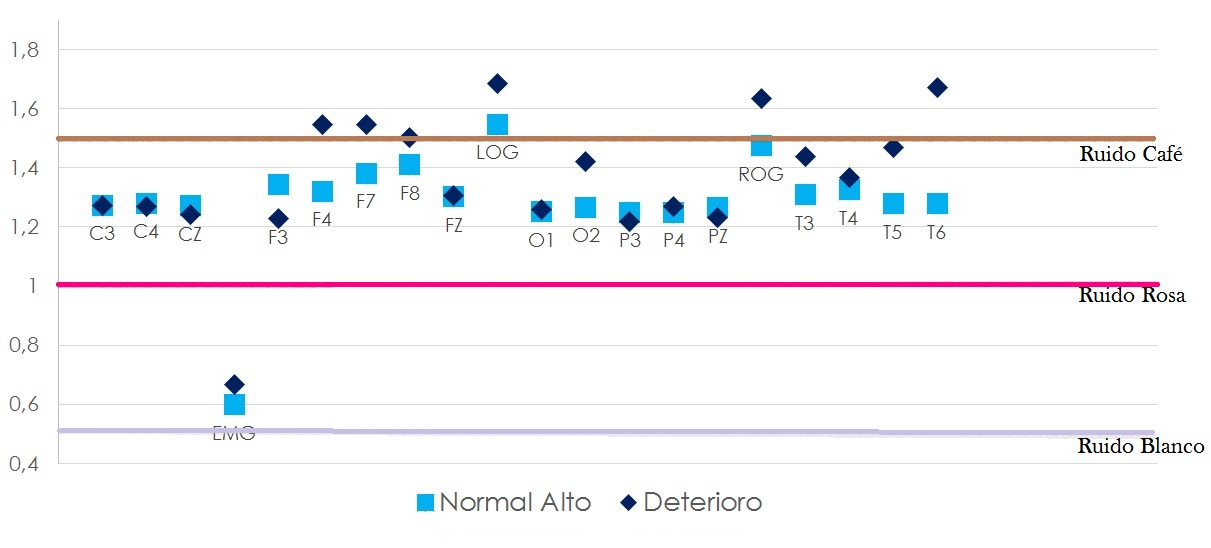
\includegraphics[scale=0.5]{comp1_3.jpg}
\caption{Aproximaci\'on del color del ruido de los resultados de DFA dadas 10 \'epocas MOR}
\label{fig:c1_3}
\end{figure}

%-----------------RELACI\'ON INTERHEMISF\'ERICA---------------------
\section{Color del ruido de la relaci\'on interhemisf\'erica}

%PENDIENTE
 En la figura \ref{fig:c2} se presentan los resultados obtenidos del an\'alisis mDFA realizado en una \'epoca de sue\~no MOR del participante con deterioro cognitivo versus sin deterioro. Donde se puede observar de una manera m\'as clara la tendencia que presenta cada caso.\\

Es decir, en el adulto mayor con deterioro cognitivo los resultados se acercan m\'as al color caf\'e, $\alpha\approx 1.5$, sin en cambio en los resultados del adulto mayor sin deterioro se mantienen pr\'oximos al ruido rosa, $\alpha\approx 1$. Y como en la secci\'on anterior se observ\'o, los resultados de LOG y ROG siguen por encima del ruido caf\'e ($\alpha\approx 1.5$).

\begin{figure}[H]
\centering
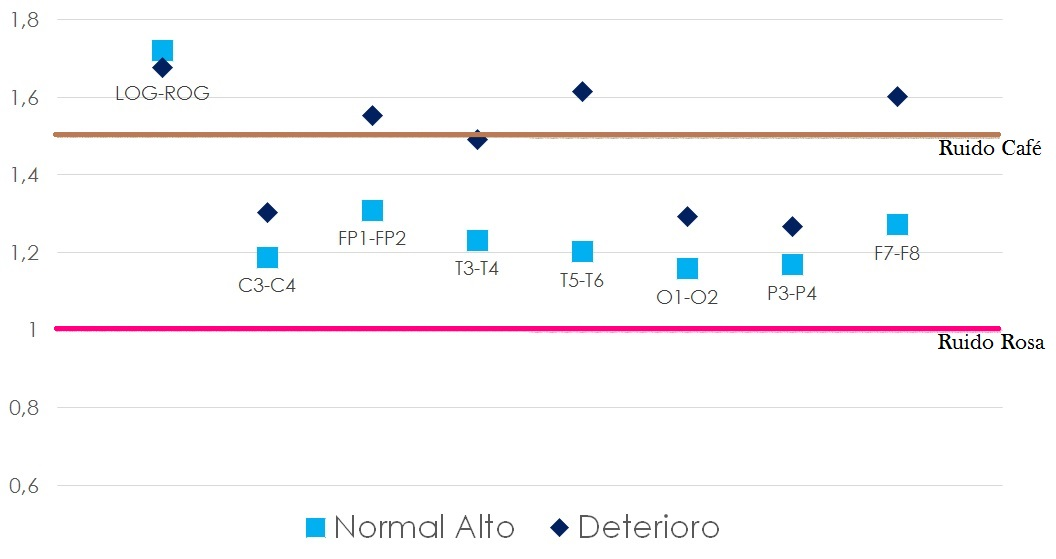
\includegraphics[scale=0.7]{comp2_1.jpg}
\caption{Aproximaci\'on del color del ruido del an\'alisis mDFA de relaciones interhemisf\'ericas}
\label{fig:c2}
\end{figure}

Considerando de nuevo el promedio de los resultados del an\'alisis mDFA de las primeras 10 \'epocas MOR de cada adulto mayor en la gr\'afica de barras que se muestra en la figura \ref{fig:c3} todos los resultados del adulto mayor con deterioro cognitivo son m\'as altos que los que se presentan en el participante sin deterioro cognitivo.\\
%M�s a�n en la relaci�n interhemisf�rica C3-C4 y P3-P4 la diferencia de ambos resultados es despreciable a comparaci�n de las dem�s. \\

Por otro lado los resultados del adulto sin deterioro cognitivo se mantienen entre los valores asignados al ruido rosa y caf\'e, con una aproximaci\'on al ruido rosa, excepto en la relaci\'on LOG-ROG. Mientras que para los valores obtenidos del adulto mayor con deterioro cognitivo la tendencia al ruido caf\'e es m\'as notable.\\

\begin{figure}[H]
\centering
\includegraphics[scale=0.5]{comp2_3.jpg}
\caption{Aproximaci\'on del color del ruido de los resultados interhemisf\'ericos dadas 10 \'epocas MOR}
\label{fig:c3}
\end{figure}

En la figura \ref{fig:c4} se encontraron diferencias estad\'isticamente significativas en el sue\~no MOR entre los grupos con deterioro cognitivo (N=3) y sin deterioro cognitivo (N=2) en los siguientes pares de derivaciones F3-F4, F7-F8, T3-T4 y P3-P4, lo cual coincide con estudios que encuentran mayores exponentes de Hurst en gente m\'as longeva, en la que tiende a ser mayor el nivel de ruido caf\'e.
\begin{figure}[H]
\centering
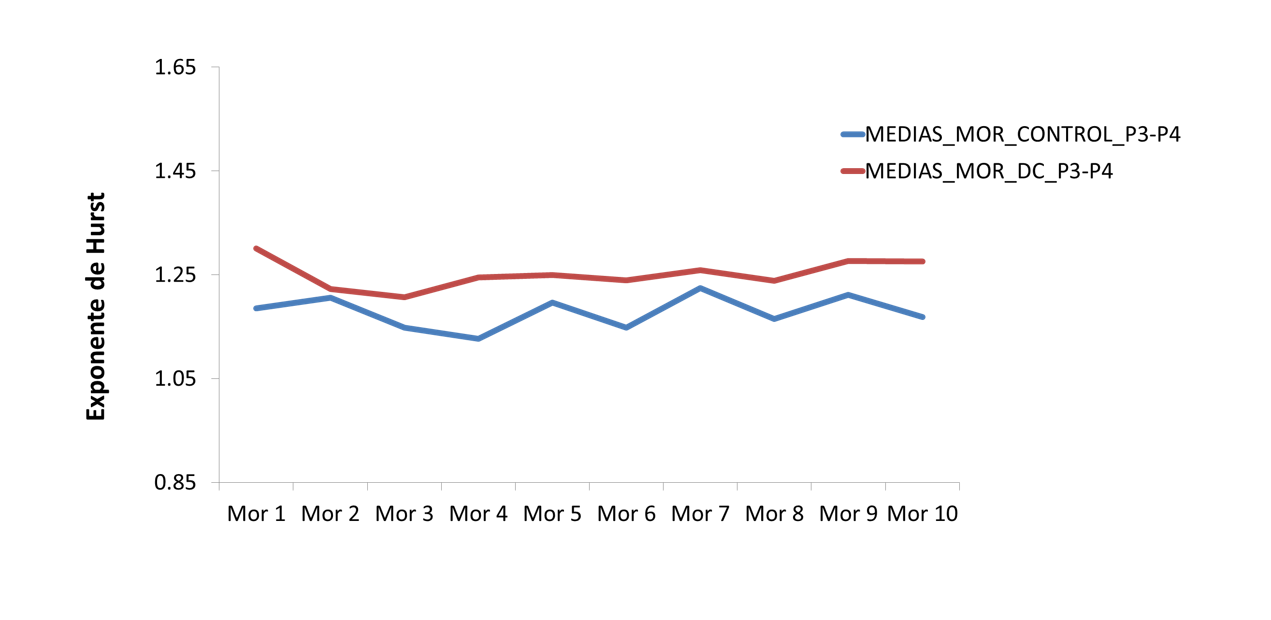
\includegraphics[scale=0.5]{com.png}
\caption{Diferencias significativas entre los grupos con deterioro y sin deterioro cognitivo de la relaci\'on P3-P4. Adaptado de \cite{Genesis}}
\label{fig:c4}
\end{figure}

%---------------CONCLUSI\'ON------------------------------

\chapter{Conclusiones}

Los resultados del modelo matem\'atico DFA se han encontrado diferencias en el sue\~no MOR de adultos mayores con y sin deterioro cognitivo. Como son:
\begin{itemize}
\item Las se\~nales de adulto mayor con deterioro cognitivo mostraron una tendencia hacia el ruido caf\'e ($\alpha\approx 1.5$).
\item Las se\~nales del adulto mayor sin deterioro cognitivo permanecieron m\'as cercanas ruido rosa ($\alpha\approx 1$). 
\item En  los registros con y sin deterioro cognitivo, la se\~nal registrada por el m\'usculo submentoniano (EMG), mostr\'o un comportamiento al ruido blanco ($\alpha\approx 0.5$), es decir, que la actividad muscular presenta todos los colores o bien, es una se\~nal aleatoria, sin importar si la persona tiene o no deterioro cognitivo.
\end{itemize}

La aplicaci\'on del an\'alisis mDFA al estudio del sue\~no MOR en los grupos de adultos mayores con y sin deterioro cognitivo muestra ciertas diferencias diferencias entre las relaciones interhemisf\'ericas de los pares F3-F4, F7-F8, T3-T4 y P3-P4, reflejando una tendencia al ruido caf\'e ($\alpha\approx 1.5$) en el adulto mayor con deterioro cognitivo y en el adulto mayor sano los resultados obtenidos tienen una mayor uniformidad y cercan\'ia al ruido rosa ($\alpha\approx 1$).\\

Los resultados obtenidos en este trabajo, pueden ser una gu\'ia para comenzar un estudio m\'as exhaustivo sobre la relaci\'on que tiene el sue\~no MOR con la memoria, implicando la relaci\'on del mismo con el deterioro cognitivo.\\

El an\'alisis de DFA y mDFA tambi\'en se puede implementar para otros estudios en series de tiempo biol\'ogicas donde el color del ruido 

%---------AP\'ENDICE--------
\chapter*{Ap\'endice}
\addcontentsline{toc}{section}{\bf Ap\'endice}

\section{Programa para \'epocas de sue\~no MOR}

Las se\~nales obtenidas en la polisomnograf\'ia al ser difitalizadas, el programa para ordenador "Registro de sue\~no" las guarda con formato .txt, sin embargo para el software MATLAB es recomendable que las se\~nales tengan formato .mat, para realizar este proceso en los 22 canales a la vez se uso el programa txtTOmat que debe pertenecer a la carpeta en la que se encuentran las 22 se\~nales y en caso de que est\'en incompletas se comentaran las faltantes.\\

Para el funcionamiento de txtTOmat, se debe de escribir el nombre que tienen las se\~nales antes del nombre que tiene cada electrodo entre comillas simples, es decir si el nombre es ``CLMNC3'' se escribir\'a 'CLMN' entre comi-llas simples o bien si es ``CLMN\_C3'' corresponde teclear 'CLMN\_ ' entre comillas simples. A continuaci\'on se presenta el programa:\\

{\tt
\setlength{\parindent}{0pt}name=\textcolor[cmyk]{0,1,0,0}{'CLMN\_'};\\
\%C3\\
strng=[name \textcolor[cmyk]{0,1,0,0}{'C3' '.txt'}];\\
C3=load(strng);\\
strng=[name \textcolor[cmyk]{0,1,0,0}{'C3' '.mat'}];\\
save(strng,\textcolor[cmyk]{0,1,0,0}{'C3'});\\
}

Lo mismo se realiza para los 21 canales restantes.\\

El anterior programa es opcional, ya que permite que en una indicaci\'on se haga el cambio de formato de los canales con una sola indicaci\'on. 

\section{Programa DFA}

El programa para el an\'alisis del DFA consta de 3 elementos que deben pertenecer a la misma carpeta en la que se encuentran los registros de sue\~no MOR o la serie de tiempo a analizar.\\

Es importante tomar en cuenta las siguientes indicaciones para un funcionamiento efectivo:
\begin{enumerate}
\item[\bf i)] El tama\~no de la serie de tiempo o cantidad de datos debe ser mayor de 2000. 
\item[\bf ii)] Los datos deber tener estar organizados en un vector columna.
\end{enumerate}

\subsection{DFA}

{\tt \setlength{\parindent}{0pt}{\textcolor{blue}{function}} output1=DFA (DATA,win\_lenght,order)\\
N=length(DATA);\\
n=floor(N/win\_length);\\
N1=n*win\_length;\\
y=zeros(N1,1);\\
Yn=zeros(N1,1);\\
fitcoef=zeros(n,order+1);\\
mean1=mean(DATA(1:N1));\\
\textcolor{blue}{for} i=1:N1\\
y(i)=sum(DATA(1:i)-mean1)\\
\textcolor{blue}{end}\\
y=y';\\
\textcolor{blue}{for} j=1:n\\
fitcoef(j,:)=polyfit(1:win\_length,y(((j-1)*win\_length+1):\\
j*win\_length),order);\\
\textcolor{blue}{end}\\
\textcolor{blue}{for} j=1:n\\
Yn(((j-1)*win\_length+1):j*win\_length)=polyval(fitcoef(j,:),\\
1:win\_length);\\
\textcolor{blue}{end}\\
sum1=sum((y'-Yn).\^2)/N1;\\
sum1=sqrt(sum1);\\
output1=sum1;\\
}

%\subsection{corrida\_DFA}
%
%
%{\tt \setlength{\parindent}{0pt} cual=ncR04;\\
%\\
%figure\\
%subplot 211\\
%\\
%plot(cual(:,1));\\
%title(\textcolor[cmyk]{0,1,0,0}{'Sue�o MOR'},\textcolor[cmyk]{0,1,0,0}{'FontSize'},16)\\
%xlabel(\textcolor[cmyk]{0,1,0,0}{'puntos'},\textcolor[cmyk]{0,1,0,0}{'FontSize'},12)\\
%ylabel(\textcolor[cmyk]{0,1,0,0}{'amplitud'},\textcolor[cmyk]{0,1,0,0}{'FontSize'},12)\\
%%xlim([1000 15000])\\
%%ylim([-.8E-5 .000015])\\
%\\
%subplot 212\\
%\\
%plot(cual(:,2));\\
%title(\textcolor[cmyk]{0,1,0,0}{'Sue�o MOR'},\textcolor[cmyk]{0,1,0,0}{'FontSize'},16)\\
%xlabel(\textcolor[cmyk]{0,1,0,0}{'puntos'},\textcolor[cmyk]{0,1,0,0}{'FontSize'},12)\\
%ylabel(\textcolor[cmyk]{0,1,0,0}{'amplitud'},\textcolor[cmyk]{0,1,0,0}{'FontSize'},12)\\
%%xlim([1000 15000])\\
%%ylim([-.8E-5 .000015])\\
%\\
%file=ncR04;\\
%
%[d\_ncR04, a\_ncR04,Fn\_ncR04]=DFA\_main(file(1000:15000,1));\\
%}

\subsection{DFA\_main}

Aqu\'i se muestran los resultados para el an\'alisis de DFA los cuales se interpretan de la siguiente manera:
\begin{itemize}
\item[\bf A:] corresponde al valor alpha ($\alpha$).
\item[\bf D:] se refiere a la dimensi\'on de la serie de tiempo.
\item[\bf n:] son los valores dados en el programa, los cuales pueden cambiar de acuerdo al an\'alisis que se har\'a.
\end{itemize}

A continuaci\'on el programa:\\

{\tt \setlength{\parindent}{0pt} \textcolor{blue}{function} [D,Alpha1,F\_n]=DFA\_main(DATA)\\
\\
n=[6,7,8,9,10,11,12,13,14,16,17,19,20,22,24,26,29,31,34,37,40,44,48,
52,57,62,68,74,81,88,96,105,114,124,136,148,161,176,191,209,228,249,
272,296,323,352,384,419,457,498,543,592,645,704,768,838,913,996,1086,
1184,1292,1409,1536,1675,1827,1992,2172,2369,2583,2817,3072,3350,3653,
3864,4344,4708,5166,5634,6144,6700,7306,7968,8689,9474]
\\
N1=length(n);\\
F\_n=zeros(N1,1);\\
\textcolor{blue}{for} i=1:N1\\
F\_n(i)=DFA(DATA,n(i),2);\\
\textcolor{blue}{end}\\
n=n';\\
 %figure;
 %plot(log10(n),log10(F_n));
%xlabel('n')
%ylabel('F(n)')
A=polyfit(log10(n(1:end)),log10(F\_n(1:end)),1);\\
Alpha1=A(1);\\
D=3-A(1);\\
\textcolor{blue}{return}\\
}

\section{Programa mDFA}

\subsection{DFA2}

{\tt \setlength{\parindent}{0pt} \textcolor{blue}{function} output1=DFA2(DATA1,DATA2,win\_length,order)\\   
N1=length(DATA1);\\
n=floor(N1/win\_length);\\
N11=n*win\_length;\\
y1=zeros(N11,1);\\
Yn1=zeros(N11,1);\\     
fitcoef1=zeros(n,order+1);\\
mean11=mean(DATA1(1:N11));\\
\textcolor{blue}{for} i=1:N11\\
y1(i)=sum(DATA1(1:i)-mean11);\\
\textcolor{blue}{end}\\
y1=y1';\\
\textcolor{blue}{for} j=1:n\\
fitcoef1(j,:)=polyfit(1:win\_length,y1(((j-1)*win\_length+1):\\
j*win\_length),order);\\
\textcolor{blue}{end}\\
\textcolor{blue}{for} j=1:n\\
Yn1(((j-1)*win\_length+1):j*win\_length)=polyval(fitcoef1(j,:),\\
1:win\_length);\\
\textcolor{blue}{end}\\
\textcolor[cmyk]{1,0,1,0}{\% PARA LA 2DA SENAL}\\
N2=length(DATA2);\\
n=floor(N2/win\_length);\\
N12=n*win\_length;\\
Yn2=zeros(N1,1);\\      
fitcoef2=zeros(n,order+1);\\
mean12=mean(DATA2(1:N12));\\
\textcolor{blue}{for} i=1:N12\\
y2(i)=sum(DATA2(1:i)-mean12);\\
\textcolor{blue}{end}
y2=y2';\\
\textcolor{blue}{for} j=1:n\\
fitcoef2(j,:)=polyfit(1:win\_length,y2(((j-1)*win\_length+1):\\
j*win\_length),order);\\
\textcolor{blue}{end}\\
\textcolor{blue}{for} j=1:n\\
Yn2(((j-1)*win\_length+1):j*win\_length)=polyval(fitcoef2(j,:),1:win\_length);\\
\textcolor{blue}{end}\\
sum1=sum( ((y1'-Yn1)).\^2);\\%/N11; %-(y2'-Yn2)
sum2=sum( ((y2'-Yn2)).\^2);\\%/N11;
sum1=sqrt((sum1+ sum2)/N11);\\
output1=sum1;\\
}

\subsection{DFA\_main2}

As\'i como en DFA\_main los resultados de este programa para el an\'alisis de DFA multicanal se interpretan de la siguiente manera:
\begin{itemize}
\item[\bf A:] corresponde al valor alpha ($\alpha$) de la relaci\'on entre dos canales.
\item[\bf D:] se refiere a la dimensi\'on de la serie de tiempo.
\item[\bf n:] son los valores dados en el programa, los cuales pueden cambiar de acuerdo al an\'alisis que se har\'a.
\end{itemize}

Donde el programa DFA\_main2 es el siguiente:\\

{\tt \setlength{\parindent}{0pt} \textcolor{blue}{function} [F\_n]=DFA\_main2(DATA1,DATA2)\\
n=[4,5,6,7,8,9,10,11,12,13,15,16,17,19,21,23,25,27,29,32,35,37,40,45,49,
54,59,64,70,75,77,83,90,108,117,128,140,152,166,181,197,215,235,256,279,
304,332,362,395,431,470,512,558,609,664,724,790,860,939,1024,1116,1218,
1328,1448,1579,1722,1878,2048,2233,2435];\\%n=108:100:2440; %8000pts a=1.0215 L6i;y 9000pts a=1.9954 L6i;  fs=1670pts/sec n=108:100:2440; 
N1=length(n);\\
F\_n=zeros(N1,1);\\
\textcolor{blue}{for} i=1:N1\\
F\_n(i)=DFA2(DATA1,DATA2,n(i),1);\\
\textcolor{blue}{end}\\
\textcolor{blue}{return}\\
}

\section{Programa para la obtenci\'on de DFA y mDFA de una \'epoca de sue\~no MOR}

Los programas mencionados en las secciones 7.2 y 7.3 pueden ser utilizados de manera individual y obtener un an\'alisis a la vez. Debido a la cantidad de datos y registros a analizar en el presente estudio se hizo uso del programa ObtenerDFA que permite el an\'alisis DFA y mDFA de una \'epoca de sue\~no MOR en los 22 canales.\\

El siguiente programa puede ser modificado de acuerdo a lo que se este analizando, en este estudio por cada \'epoca el tiempo para la obtenci\'on de todos los datos fue de aproximadamente 2 horas, durante las cuales se pueden realizar otras actividades.\\

As\'i como los anteriores programas, \'este debe estar en la misma carpeta que los anteriores as\'i como en el caso de faltar alg\'un canal, \'este debe ser comentado donde sea mencionado en el programa, donde los datos que se deben teclear corresponden a lo siguiente:
\begin{itemize}
\item {\bf name=} As\'i como en txtTOmat se debe colocar el nombre de las se\~nales, que est\'an del canal.
\item {\bf Etapa=} \'Epoca que expertos han catalogado como \'epoca de sue\~no MOR.
\item {\bf Hz=} Frecuencia de la serie de tiempo, o bien n\'umero de repeticiones por unidad de tiempo.
\end{itemize}

{\tt \setlength{\parindent}{0pt}name=\textcolor[cmyk]{0,1,0,0}{'CLMN\_'};\\
Etapa=140;\\
Hz=512;\\
x=1+(Etapa-1)*30*Hz;\\
y=Etapa*30*Hz;\\
C3\_S=C3(x:y);\\
C4\_S=C4(x:y);\\
\textcolor[cmyk]{1,0,1,0}{\%Lo mismo se realiza para los dem\'as canales.}\\
n=[4 5 6 7 8 9 10 11 12 13 15 16 17 19 21 23 25 27 29 32 35 37 40 45 49 54 59 64 70 75 77 83 90 108 117 128 140 152 166 181 197 215 235 256 279 304 332 362 395 431 470 512 558 609 664 724 790 860 939 1024 1116 1218 1328 1448 1579 1722 1878 2048 2233 2435];\\
n=n';\\
log\_n=log(n);\\
expnt=[];\\

}
{\tt \setlength{\parindent}{0pt}[Fn\_c3c4]=DFA\_main2(C3\_S,C4\_S)\\
log\_Fn=log(Fn\_c3c4);\\
p=polyfit(log\_n,log\_Fn,1);\\
m\_c3c4=p(1);\\
expnt=[expnt;m\_c3c4];\\}

\textcolor[cmyk]{1,0,1,0}{\%Lo cual se realiza para el resto de las relaciones interhemisf\'ericas.}\\

{\tt \setlength{\parindent}{0pt}alpha=[];D=[];\\}
{\tt \setlength{\parindent}{0pt}[Dc3,Alphac3,F\_nc3]=DFA\_main(C3\_S);\\
D=[D;Dc3];\\
alpha=[alpha;Alphac3];\\}
\textcolor[cmyk]{1,0,1,0}{\%La misma acci\'on se realiza para obtener el an\'alisis DFA de los dem\'as canales.}\\

{\tt \setlength{\parindent}{0pt}save([\textcolor[cmyk]{0,1,0,0}{'variables'} name \textcolor[cmyk]{0,1,0,0}{'.mat'}])\\}

Con este programa los resultados se obtendr\'an de la siguiente manera:
\begin{itemize}
\item {\bf Alpha:} Los $\alpha$ de cada canal, es decir, los resultados del an\'alisis DFA de cada canal.
\item {\bf D:} Dimensi\'on fractal de cada canal.
\item {\bf expnt:} El valor $\alpha$ de cada relaci\'on interhemisf\'erica (Resultados del an\'alisis mDFA).
\end{itemize} 

%-------------BIBLIOGRAF�A------------------------------

%\chapter{Bibliograf�a}

\begin{thebibliography}{10}

%\cleardoublepage
\addcontentsline{toc}{section}{\bf Bibliograf\'ia}

\bibitem{Baltes}
Baltes, P. B. (1987). Theoretical propositions of life-span developmental psychology: On the dynamics between growth and decline. Developmental psychology, 23(5), 611.

\bibitem{Bonet}
Bonet, T. (2008). Bases anat\'omicas y fisiol\'ogicas del sue\~no. Universidad de Valencia.

\bibitem{Conde}
Conde, A. F., \& S\'anchez, E. V. (2007). El sue\~no en el anciano. Atenci\'on de enfermer\'ia. Enfermer\'ia global, 6(1).

\bibitem{sue}
Chokroverty, S. (2009). Sleep disorders medicine: basic science, technical considerations, and clinical aspects. Elsevier Health Sciences.

\bibitem{Frac}
Feder, J. (1988). Fractals, 1988.

\bibitem{Goldberger}
Goldberger, A. L., Amaral, L. A., Glass, L., Hausdorff, J. M., Ivanov, P. C., Mark, R. G., ... \& Stanley, H. E. (2000). Physiobank, physiotoolkit, and physionet components of a new research resource for complex physiologic signals. Circulation, 101(23), e215-e220.

\bibitem{Goldberge}
Goldberger, A. L., Amaral, L. A., Hausdorff, J. M., Ivanov, P. C., Peng, C. K., \& Stanley, H. E. (2002). Fractal dynamics in physiology: alterations with disease and aging. Proceedings of the National Academy of Sciences, 99 (suppl 1), 2466-2472.

\bibitem{ING}
http://www.geriatria.salud.gob.mx/  (2016)

\bibitem{Estec}
Lind, D. A., Marchal, W. G., \& Wathen, S. A. (2005). Estad\'istica aplicada a los negocios y la econom\'ia. McGraw-Hill,.

\bibitem{Est}
Mendenhall, W., Scheaffer, R., \& Wackerly, D. (1986). Estad\'istica Matem\'atica con Aplicaciones, 7ma. Edici\'on Grupo Editorial Iberoam\'erica.

\bibitem{Miramontes}
Miramontes, P. (1999). El color del ruido. Ciencias, (054).

\bibitem{OMS}
Crecimiento acelerado de la poblaci\'on adulta de 60 a\~nos y m\'as de edad: Reto para la salud p\'ublica. (http://www.paho.org)(2016)

\bibitem{cartel}
Garc\'ia Mu\~noz V., Rodr\'iguez-Torres EE, Itz\'a Ortiz BA, Viveros Rogel J, L\'opez-Garc\'ia K, y Jim\'enez-Estrada I. M\'etodo de Correlaci\'on Integraci\'on Fractal aplicado a Fibras Musculares. Congreso Nacional, Sociedad Mexicana de Ciencias Fisiol\'ogicas 2015, San Miguel Allende, Guanajuato M\'exico.

\bibitem{Peng}
Peng, C. K., Havlin, S., Stanley, H. E., \& Goldberger, A. L. (1995). Quantification of scaling exponents and crossover phenomena in nonstationary heartbeat time series. Chaos: An Interdisciplinary Journal of Nonlinear Science, 5(1), 82-87.

\bibitem{Rincon}
Rinc\'on, L., \& Correa, A. F. J. M. (2007). Probabilidad y Estad\'istica. Ciudad de M\'exico: Facultad de Ciencias UNAM.

\bibitem{mDFA}
Rodr\'iguez, E. E., Hern\'andez-Lemus, E., Itz\'a-Ortiz, B. A., Jim\'enez, I., \& Rudom\'in, P. (2011). Multichannel detrended fluctuation analysis reveals synchronized patterns of spontaneous spinal activity in anesthetized cats. PLoS One, 6(10), e26449.

\bibitem{carteloli}
Rodr\'iguez Torres EE, Res\'endiz Flores O, Viveros Rogel J, Leonel G\'omez R, Pablo Rudomin. An\'alisis de Caos en Series de Tiempo de la Actividad Espont\'anea de Conjuntos Neuronales en la M\'edula Espinal del Gato. Congreso Nacional, Sociedad Mexicana de Ciencias Fisiol\'ogicas 2015, San Miguel Allende, Guanajuato M\'exico.

\bibitem{DC}
Rosselli, M., \& Ardila, A. (2012). Deterioro Cognitivo Leve: Definici\'on y Clasificaci\'on.

\bibitem{et_sue}
Secretar\'ia de Salud de M\'exico. Diagn\'ostico y tratamiento de los Transtornos del Sue\~no. M\'exico, 2009http://www.isssteags.gob.mx/guias\_practicas\_medicas/gpc/docs/
IMSS-385-10-RR.pdf (accedido 18 feb 2016) 

\bibitem{Sierra}
Sierra, J. C., Jim\'enez-Navarro, C., \& Mart\'in Ortiz, J. D. (2002). Calidad del sue\~no en estudiantes universitarios: importancia de la higiene del sue\~no. Salud mental, 25(6), 35-43.

\bibitem{Vas}
Vassalli, A., \& Dijk, D. J. (2009). Sleep function: current questions and new approaches. European Journal of Neuroscience, 29(9), 1830-1841.

\bibitem{Genesis}
V\'azquez Tagle Gallegos G\'enesis del Roc\'io, Garc\'ia Mu\~noz Valeria, Rodr\'iguez Torres Erika Elizabeth, Pliego Pastrana Patricia, Mart\'inez-Alcal\'a Claudia, Rosales-Lagarde Alejandra. Correlaci\'on interhemisf\'erica durante el sue\~no MOR del adulto mayor con deterioro cognitivo. LIX Congreso Nacional de Ciencias Fisiol\'ogicas. 14 \& 18 de agosto de 2016. Campeche, Camp. M\'exico.

\end{thebibliography}

\end{document}
